% ======================================================== %
% Przeczytaj plik amuthesis-doc.pdf, aby poznać opcje      %
% klasy `amuthesis`                                        %
% ======================================================== %
\documentclass[oneside,polski,logo]{amuthesis}

% Zdefiniuj kodowanie pliku źródłowego (domyślnie utf8)
\usepackage[utf8]{inputenc}
\usepackage[nottoc,notlot,notlof]{tocbibind}
\usepackage{hyperref}

% ======================================================== %
% Dane autora i pracy                                      %
% ======================================================== %

% --- Autor pracy
\author{Kamil Tyrek, Mateusz Hypś, Jakub Kozubal}
% --- Numer albumu
\album{434797, 434699, 434726}
% --- Tytuł pracy (w języku polskim i angielskim)
\titlePL{Projekt i implementacja gry „The Lore: Story of the fallen warrior”}
\titleEN{Project and implementation of game „The Lore: Story of the fallen warrior”}
% --- Typ pracy (inżynierska, licencjacka, magisterska)
\type{inżynierska}
\graphicspath{ {./images} }
% --- Wydział (wykaz skrótów):
% --- --- WA    --- Wydział Anglistyki
% --- --- WB    --- Wydział Biologii
% --- --- WCh   --- Wydział Chemii
% --- --- WFPiK --- Wydział Filologii Polskiej i Klasycznej
% --- --- WF    --- Wydział Fizyki
% --- --- WH    --- Wydział Historyczny
% --- --- WMiI  --- Wydział Matematyki i Informatyki
% --- --- WNGiG --- Wydział Nauk Geograficznych i Geologicznych
% --- --- WNPiD --- Wydział Nauk Politycznych i Dziennikarstwa
% --- --- WNS   --- Wydział Nauk Społecznych
% --- --- WN    --- Wydział Neofilologii
% --- --- WPAK  --- Wydział Pedagogiczno-Artystyczny w Kaliszu
% --- --- WPiA  --- Wydział Prawa i Administracji
% --- --- WSE   --- Wydział Studiów Edukacyjnych
% --- --- WT    --- Wydział Teologiczny
% --- --- IKE   --- Instytut Kultury Europejskiej w Gnieźnie
\faculty{WMiI}
% --- Kierunek (w mianowniku)
\field{informatyka}
% --- Specjalność (w formie mianownikowej)
% --- (ustaw puste, jeśli bez specjalności)
% --- Promotor (w dopełniaczu)
\supervisor{dr Bartłomieja Przybylskiego}
% --- Data złożenia pracy (Miasto, miesiąc rok)
\date{Poznań, luty 2021}

% --- Płeć autora (M/K)
\stsex{M}
% --- Zgoda na udostępnienie pracy w czytelni (TAK/NIE)
\stread{TAK}
% --- Zgoda na udostępnienie pracy w zakresie ochrony (TAK/NIE)
\stprotect{TAK}
% --- Data podpisania oświadczenia (Miasto, data)
\stdate{Poznań, \today{} r.}

% ======================================================== %
% Dodatkowe pakiety wykorzystywane w pracy                 %
% ======================================================== %

\usepackage{lipsum}

% ======================================================== %
% Zasadnicza część dokumentu                               %
% ======================================================== %

\begin{document}

% Strona tytułowa
\maketitle
% Streszczenie
\begin{streszczenie}
Przedmiotem pracy jest przedstawienie projektowania gry platformowej „The Lore: story of the fallen warrior” w oparciu o silnik Unity. Gra posiada elementy zręcznościowe oraz zagadki logiczne, przez co przechodzenie kolejnych etapów gry wymaga szybkiego podejmowania logicznych decyzji. \par
Na początku - nazwij jak chcesz, pamiętaj, że rozdzial 1 to wstep… Mateusz Hypś. \par
W następnym rozdziale będziemy mogli dowiedzieć się czym jest zagadka logiczna oraz poznać kilka przykładów. Opisany zostanie sposób obsadzenia mini-gier w grze opartej na silniku Unity. W kontekście projektu „The Lore”, przedstawione są algorytmy stojące za logiką zaimplementowanych mini-gier – przesuwanych puzzli, otwierania skrzyń, mini-gry z ułożeniem rur. Dodatkowo przedstawiono metodę projektowania mini-gry nie zawartej w projekcie - algorytmu generującego labirynt. \par
W ostatnim rozdziale… Jakub Kozubal

\end{streszczenie}
% Spis treści
\tableofcontents



% ======================================================== %
% Właściwa część pracy                                     %
% ======================================================== %

\chapter{Wstęp}
\section{Cel i założenia projektu}
Celem projektu jest stworzenie gry platformowej, zawierającej elementy zręcznościowe oraz łamigłówki. Głównym założeniem projektu jest gra, która zaciekawi swoją fabułą oraz trudnością. Wstępnie prosty zamysł samouczka, w większości gier jest raczej elementem wprowadzającym do rozgrywki, która powinna robić się trudniejsza w im dalszym etapie rozgrywki się znajdujemy, w przypadku naszej gry jest odwrócony. Samouczek poza wprowadzaniu poszczególnych elementów rozgrywki, którymi jest między innymi przedstawienie sterowania oraz funkcjonalności i wstępnych mechanik jest również wymagający, od gracza zależy jakie umiejętności w trakcie rozgrywki będzie rozwijać, aby przejście kolejnych poziomów było łatwiejsze (z perspektywy gracza). Dużą wagę w projekcie przywiązujemy do mini-gier, które występują w trakcie przechodzenia poszczególnych poziomów. Występują dwa rodzaje mini-gier: opcjonalne (te które przejść możemy w celu sprawdzenia siebie oraz zdobycia punktów doświadczenia) oraz wymagane, które trzeba przejść, aby znaleźć się w dalszym etapie gry. Użytkownik posiada do dyspozycji punkty doświadczenia, drzewko umiejętności oraz ekwipunek. Punkty doświadczenia możemy wydawać bezpośrednio w drzewku umiejętności, w którym zadaniem gracza jest wybranie odpowiednich umiejętności zależnie od tego jaką strategię rozgrywki chce przyjąć. Warto pamiętać jednak, że im głębiej będziemy rozwijać daną gałęź tym umiejętności będą bardziej pomocne co sprawia, że gracz musi zastanowić się dobrze nad decyzjami dotyczącymi rozwijania konkretnych umiejętności w drzewku. Ekwipunek służy do zdobywania przedmiotów potrzebnych w trakcie rozgrywki m.in. do otwierania drzwi czy rozpoczęcia opcjonalnej mini-gry. W projekcie są wykorzystane 2 style tworzenia poziomów: ortographic i perspective. Wszystkie animacje w projekcie są tworzone z użyciem technologii inverse kinematics co pozwala na stałe dodawanie nowych animacji i poprawianie już istniejących.
\section{Organizacja pracy}
Charakter projektu sprawił, iż nie można w naszym zespole jasno podzielić typów zadań, które realizujemy w ramach projektu. Wynikiem tego jest to, iż nowe funkcjonalności są realizowane zazwyczaj przez jedną osobę od początku do końca, nie ma podziału, podobnego jak w przypadku aplikacji z frontendem i backendem.


Jako metodykę pracy przyjęto Scrum. Głównymi powodami tej decyzji jest doświadczenie części zespołu w tej metodyce oraz przejrzystość i rozsądne zarządzanie pracą. Nie rozważano innych metodyk pracy. Przy zarządzaniu pracą wspomaga nas serwis JIRA, który pozwala zarządzać regularne sprinty – w pierwszym semestrze dwutygodniowe, w drugim semestrze tygodniowe. 


Kod źródłowy zarządzany jest poprzez GitHub. Dla przejrzystości pracy, każdy commit na GitHub oznaczany jest id zadania na Jirze, dzięki czemu wchodząc w zadanie widzimy commit powiązany z jego rozwiązaniem. W momencie rozpoczęcia zadania deweloper, jeśli następuje potrzeba, tworzy podzadania do zadań na Jirze. Dotyczy to większych zadań, których wykonanie polega na tworzeniu większej ilości funkcjonalności. Dzięki temu realizując nowe zadania, o podobnej budowie, można sugerować się podobnym sposobem działania zadania. Po każdym commicie programista wyznacza ile czasu poświęcił na zadanie, poprzez wbudowaną w Jirze funkcjonalność “Log Work”. Gdy zadanie zostanie zakończone, programista oznacza je statusem “DONE”.  


Z racji wybranej metodyki, dokonano również przydzielenia odpowiednich ról członkom zespołu. Podział ról wygląda następująco:

\begin{itemize}
	\item Kamil Tyrek - Development Team, Scrum Master
	\item Jakub Kozubal -Development Team, Product Owner
	\item Mateusz Hypś - Development Team
\end{itemize}

\section{Podział prac}
\subsection{Kamil Tyrek - tworzenie elementów logicznych i ich algorytmika}
W tym rozdziale zostaną przedstawione sposoby tworzenia elementów logicznych. Część z przedstawionych łamigłówek została użyta w projekcie końcowym. Przykładem są tutaj przesuwane puzzle - rozgrywka polegająca na przesunięciu elementu, celem ułożenia poprawnego obrazka. Algorytmika stojąca za losowaniem kolejności elementów nie jest trywialna, ponieważ źle wylosowana kolejność puzzli powoduje, iż mogą być niemożliwe do ułożenia.

Zostanie przedstawiona też logika mini-gry z ustawieniem odpowiednich ruch, celem połączenia dwóch końców rur. Podobnie jak w poprzednim przykładzie, do rozwiązania tej zagadki potrzebna jest odpowiednia liczba rur danego typu - pionowe, poziome, skrętne. 

Następnym przykładem będzie logika stojąca za rozgrywką, która nie jest dostępna w końcowym projekcje, a chodzi tutaj o generowanie labiryntu. Nietrywialnym problemem jest wygenerowanie takiej planszy, aby możliwe było przejście z punktu A do punktu B. W tym rozdziale postaramy się przedstawić rozwiązanie tego problemu, przy użyciu odpowiednich algorytmów.

\subsection{Mateusz Hypś - Zarządzanie projektem gry komputerowej z wykorzystaniem Agile}
W rozdziale zostanie opisany proces zarządzania projektem z wykorzystaniem metodyki zwinnej. Omówione i porównane zostaną podejścia Agile i Agile Game Development oraz zastosowania tych metodyk, w porównaniu z innymi stosowanymi w praktyce. Przedstawione zostaną najważniejszych idee stojące za metodykami Agile m.in. framework SCRUM. Następnie omówione zostanie zastosowanie tych metodyk w projekcie “The Lore”, z uwzględnieniem problemów w trakcie realizacji tego projektu. 
\subsection{Jakub Kozubal - Fizyka postaci}
W tym rozdziale zostaną przedstawione sposoby tworzenia poruszania się postaci. Zaznaczone zostaną główne różnice między fizyką rzeczywistą, a tą stosowaną w grach jak i przedstawienie wielu sposobów rozwiązania tej samej funkcjonalności. Ponadto przedstawiony zostanie proces tworzenia postaci. Do tego pojawi się też opisanie problemów takich jak sterowanie postaci w powietrzu oraz oddziaływanie sił z otoczenia (m.in. poruszające się platformy). Zostanie także przedstawione i przeanalizowane działanie każdej umiejętności występującej w drzewku odpowiedzialnej za poruszanie się.

\section{Użyta technologia - Unity}
 W naszym projekcie postanowiliśmy wybrać UNITY jako środowisko do stworzenia naszej gry. Wynikało to z możliwości jakie oferuje oraz z jakości i czytelności, stworzonej przez twórców, oficjalnej dokumentacji. Pozwala nam na tworzenie gier dwuwymiarowych czy trójwymiarowych oraz interaktywnych materiałów, na przykład animacje czy wizualizacje. W razie problemów możemy również wykorzystywać oficjalne forum na którym rzesza użytkowników dzieli się swoimi wskazówkami a także oficjalny sklep – Asset Store, w którym możemy wykupić materiały potrzebne do naszej gry. UNITY działa na każdym systemie operacyjnym, tj. Windows, macOS oraz Linux. Gwarantuje nam również możliwość stworzenia aplikacji nie tylko na komputery osobiste, ale także przeglądarki internetowe, konsole gier wideo oraz urządzenia mobilne. Dzięki aktualizacji silnika do wersji 5.1.1 ta lista wzrasta do 22 platform sprzętowych, w tym gogle wirtualnej rzeczywistości takie jak Oculus Rift.
W przeszłości można było tworzyć aplikacje w trzech językach:
\begin{itemize}
	\item UnityScript (swego rodzaju pochodna JavaScript’u)
	\item C\#
	\item Boo
\end{itemize}
Jednak wraz z piątą wersją silnika (wydaną w roku 2015) możliwość pisania w języku Boo została usunięta, pozostała tylko wsteczna kompatybilność w postaci możliwości kompilacji skryptów przez środowisko MonoDevelop. Podobny los dotknął UnityScript, którego wsparcie zakończyło się na wersji 2018.2 (najnowsza wersja stabilna to 2019.3.4). Z tych względów nasz wybór musiał paść na język C\#, w którym zostały napisane wszystkie nasze skrypty. Jako jedyny jest wciąż wspierany przez autorów, co zaowocowało drastycznym wzrostem popularności wśród użytkowników.

\chapter{Zarządzanie projektem gry komputerowej z wykorzystaniem Agile}
\section{Czym jest projekt?}
Aby odpowiednio przyswoić temat zarządzenia projektem, należy zacząć od zrozumienia paru terminów  które są nieodłączną jego częścią. \\ \\
Projekt jest to termin z pozoru banalny, w końcu spotykamy się z nim wielokrotnie, jednak wytłumaczenie go może sprawiać problemy. Jedną z najlepszych oraz najbardziej wyczerpujących definicji na jaką można trafić jest ta stworzona przez Roberta K. Wysockiego oraz Rudd’a McGary'ego. Są to Amerykańscy specjaliści w temacie zarządzania projektami. W ich książce pod tytułem „Efektywne zarządzanie projektami” definiują projekt jako: „sekwencję niepowtarzalnych, złożonych i związanych ze sobą zadań, mających wspólny cel, przeznaczonych do wykonania w określonym terminie bez przekraczania ustalonego budżetu, zgodnie z założonymi wymaganiami”. \cite{projekt} \\

Pomimo faktu iż powyższa definicja jest najprawdopodobniej znacznie bardziej złożona od takiej którą słyszymy na co dzień to jest ona bardzo cenna, ponieważ przedstawia najważniejsze cechy każdego projektu.\\

Składa się z czterech podstawowych elementów, którymi menedżer projektu musi zarządzać symultanicznie. Trzeba pamiętać, że są one ze sobą powiązane. Do wspomnianych elementów należą: 
\begin{itemize}
	\item Zakres
	\item Zasoby
	\item Czas
	\item Pieniądze
\end{itemize}

\subsection {Zakres}
Zdecydowanie najważniejszy z całej czwórki. Jest on definicją co tak naprawdę projekt ma osiągnąć i co ma w nim zostać zrealizowane. Obrazuje rozmiar projektu, jego cele a także wymagania. Zakres jest nie tylko najważniejszym, ale również najbardziej złożonym. Jakakolwiek zmiana musi zostać odwzorowana w pozostałych trzech elementach. Jest to jeden z powodów dla którego się mówi o współzależności między tą czwórką. Aby to lepiej zrozumieć, można sobie wyobrazić aplikacje, która ma posiadać cztery główne funkcjonalności, zbudowana przez dwa zespoły z budżetem 40 tysięcy złotych. Jeśli zakres projektu się zmieni do przykładowo sześciu funkcjonalności, zadaniem menedżera projektu jest dostosowanie zasobów ludzkich, czasu oraz budżetu w taki sposób aby cel ten został zrealizowany.

\subsection {Zasoby}
Zasoby dzielą się na trzy kategorie:
\begin{itemize}
	\item Zasoby ludzkie
	\item Wyposażenie
	\item Materiały
\end{itemize}
\subsubsection {Zasoby ludzkie}

Menadżer projektu musi upewnić się że pracownicy posiadają odpowiednie umiejętności i narzędzia aby ukończyć dane im zadanie. Musi w pełni monitorować czy ma wystarczającą ilość zasobów ludzkich do konkretnego projektu tak aby go ukończyli w ustalonym czasie. Jego zadaniem jest również dopilnowanie aby każda osoba przypisana do zadania doskonale wiedziała i rozumiała co ma zrobić oraz znała wyznaczone terminy. W większych firmach wygląda to inaczej. Pracownicy są podzieleni na grupy którymi zarządza team leader, jest on odpowiedzialny za większość obowiązków które zostały wymienione powyżej. Wynika to z faktu iż menedżer projektu nie jest w stanie zarządzać tak dużym zbiorowiskiem ludzi. Dużym atutem jest również to że team leader najlepiej zna swój zespół, ich umiejętności, możliwości, a także czas którym dysponują. Jest to również duże ułatwienie dla menedżera projektów ponieważ nie musi komunikować się ani nadzorować wszystkich, wystarczy kontakt z team leaderem konkretnych zespołów. 

\subsubsection {Wyposażenie i materiały}
Czasami dochodzi do sytuacji, w której project manager jest odpowiedzialny za pozyskiwanie materiałów i wyposażenie którymi musi zarządzać w taki sposób aby zespół wykonywał swoją prace w najefektywniejszy sposób. Nie jest to często spotykane zjawisko, w szczególności w dużych firmach w których podzial obowiązków jest mocniej rozdzielony po wielu pracownikach.

\subsection {Czas}
Podobnie jak w przypadku zasobów, czas jest dzielony na trzy grupy
\begin{itemize}
	\item Podział na zadania
	\item Harmonogram
	\item Ścieżka krytyczna (ang. Critical path)
\end{itemize}

\subsubsection {Podział na zadania}
Podział na zadania jest pierwszym z trzech kroków do pomyślnego zarządzania czasem. Zadania muszą być tworzone w przemyślany sposób, dobrze przeanalizowane, a także odpowiednio wytłumaczone, tak aby pracownik, który się go podejmie, wszystko zrozumiał za pierwszym razem. Niespełnienie przynajmniej jednego z wyżej wymienionych warunków tworzenia zadań negatywnie wpływa na ich wykonanie. W wielu przypadkach łączy się to z opóźnieniami w realizacji projektu.

\subsubsection {Harmonogram}
Po pomyślnym stworzeniu zadań przechodzi się do zaplanowania harmonogramu. Tworzy się go poprzez listowanie w odpowiedniej kolejności wszystkich zadań, które muszą zostać wykonane. Niektóre z nich można wykonywać sekwencyjnie, inne z nich mogą nakładać się na siebie, a jeszcze inne mogą zostać wykonane jednocześnie. Kluczem do sukcesu jest ich zrozumienie i poprawne grupowanie. Następnym ważnym czynnikiem jest zrozumienie zależności między nimi, ponieważ niektóre z zadań muszą zostać wykonane w pierwszej kolejności. Ostatnim krokiem tworzenia harmonogramy jest estymacja czasu potrzebnego do ich wykonania, a także przypisanie im odpowiednich zasobów. 

\subsubsection {Ścieżka krytyczna (ang. Critical path)}
Niektóre zadania mają elastyczny termin rozpoczęcia oraz ich zakończenia. Jednak istnieją również takie które tej elastyczności nie mają. Linia przechodząca przez zbiór takich zadań nazywana jest ścieżką krytyczną i wykorzystywana jest do monitorowania w jakim tempie zostają wykonywane zadania w projekcie. W zależności od podziału zadań, istnieje możliwość występowania wielu ścieżek krytycznych. Wszystkie zadania które znajdują się na ich drodze muszą zostać wykonane w terminie, w przeciwnym razie występuje bardzo wysokie prawdopodobieństwo że projekt nie zostanie ukończony na czas.

\subsection {Pieniądze}
Dla najefektywniejszego zarządzania kosztami projektu uwzględnia się jego:

\begin{itemize}
	\item Koszty
	\item Wydatki związane z losowymi zdarzeniami
	\item Zyski
\end{itemize}

\subsubsection {Koszty}
Każde zadanie ma określony koszt potrzebny do jego do wykonania, najczęściej bazuje na wydatkach związanych z potrzebnymi zasobami. Każdy z tych wydatków jest estymowany i uwzględniany podczas przygotowania budżetu dla projektu.

\subsubsection {Wydatki związane z losowymi zdarzeniami}
Podobnie jak w estymacji czasu potrzebnego do wykonania konkretnych zadań, tak samo przy przygotowywaniu budżetu należy uwzględnić pewien bufor. Zostanie on wykorzystany na wypadek losowych zdarzeń, które mogą się w nieoczekiwanym momencie wydarzyć. Najprostszym przykładem w firmie informatycznej może być problem techniczny związany ze sprzętem np. zepsuty komputer.

\subsubsection {Zyski}
Zyski są to pieniądze, które firma planuje zarobić na wykonanym projekcie, bądź po każdym zakończonym zadaniu. Oczywiście aby projekt został uznany za opłacalny dla biznesu, budżet, który zawiera odpowiednio oszacowane koszty nie może przekraczać pewnego procentu planowanych zysków. Zadaniem menedżera projektu jest oczywiście zminimalizowanie jak najbardziej kosztów produkcji i jak największe zmaksymalizowanie zysku, które firma zarobi po wykonanym projekcie.


\section {Czym jest zarządzanie projektem?}
Wiedząc już dokładnie czym jest projekt, zrozumienie na czym polega zarządzanie nim staje się trywialne. W dużym uproszczeniu jest to proces,  który za pomocą sprecyzowanego planu pozwala na osiągnięcie wyznaczonego przez ciebie lub twoją firmę celu. Stworzenie odpowiedniego planu, podzielonego na szereg kroków, jest tutaj znaczący, ponieważ do osiągnięcia wyznaczonego celu wymagane jest ukończenie wszystkich zadań po drodze. Bardzo często zarządzanie projektem jest porównywane do wchodzenia po schodach bądź wspinania się po drabinie. Aby osiągnąć wyznaczony cel i dojść na samą górę, trzeba krok po kroku zaliczać każdy poziom. Podobnym trafnym porównaniem jest podróż z jednego miejsca do drugiego. Należy rozpatrzeć różną trasę w celu zrozumienia, która jest z nich będzie najlepsza. Następnie wyestymować czas, potrzebny na podróż, przemyśleć sposoby w jaki się tam dostaniesz czy to pieszo czy za pomocą pojazdu. Przygotować potrzebny budżet oraz przeanalizować potencjalne zagrożenia. jak widać zarządzanie projektem nie występuje tylko w biznesie, jest to szeroko pojęte zdarzenie, które doświadczamy każdego dnia. Jednak nawet na tak prostym przykładzie, można zrozumieć jak ważny jest to aspekt naszego życia, a także jak kluczowe ma efekty w biznesie.\\

Zarządzanie projektem nie składa się tylko z planowania i pilnowania czy wszystko idzie zgodnie z założeniami. Jest to również dziedzina która ma na celu budowanie motywacji zespołu projektowego, zadbanie o właściwą komunikację między jego stronami, a także zrozumieniu ich potrzeb. W zależności od rozmiaru firmy proces taki potrafi być bardzo trudny.\\

Innym czynnikiem wchodzącym w skład zarządzania projektem jest analiza zagrożeń oraz praktyczna wiedza pozbywania się ich. Jest to tak zwana eliminacja ryzyka występująca podczas całego cyklu życia projektu. Ryzyko w projektach pochodzi głównie z niemożliwości wyeliminowania niechcianych incydentów oraz niepewności związanej z przyszłością. Do tego typu zdarzeń dochodzi na każdym kroku projektu, wynika to z dynamiki procesu, potencjalnych konfliktów między pracownikami, niespodziewanymi komplikacjami związanymi z zasobami, zmiennej wydajności pracy czy zwyczajnie błędnego planowania. Aby jak najbardziej ograniczyć ryzyko przy jednoczesnej maksymalizacji optymalizacji użycia zasobów zatrudnia się odpowiednią na to miejsce osobę, zwaną menadżerem projektu lub kierownikiem projektu. \\ \\ \\ \\ \\ \\ \\ \\ \\ \\ \\ \\ \\

\begin{figure}[h]
	\centering
	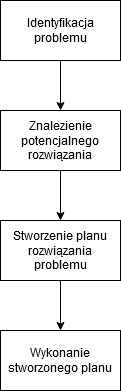
\includegraphics[width=4cm]{images/hyps/diagram-zarzadzania-projektem.png}
	\caption{Uproszczony proces realizacji projektu}
\end{figure}

Powyższy diagram obrazuje proces realizacji projektu w bardzo uproszczonym formacie, ponieważ każdy etap kryje za sobą wiele procesów które trzeba dodatkowo wykonać.\\
\section {Kim jest menedżer projektu?}
Menedżer projektu zwany również kierownikiem projektu czy PM’em od angielskiej nazwy project manager. Jest to specjalista którego główną odpowiedzialnością jest rozpoczęcie cyklu życia projektu. Zaczyna od przygotowania planu działania a następnie wdrożenia go i zrealizowania aby następnie móc zamknąć projekt z sukcesem. Jego podstawowym zadaniem jest zapewnienie wykonania wcześniej zaplanowanych celów, po to aby wydać produkt docelowy spełniający wszelkie wymagania. Kluczowymi obowiązkami są:\\

\begin{itemize}
	\item wstępne zaplanowanie projektu, a następnie jego ustandaryzowanie
	\item wprowadzenie kluczowych zasad działania
	\item opracowanie logicznych i możliwych do zrealizowania celów
	\item odpowiednie rozporządzenie czasem oraz kosztami \\
\end{itemize}

W niektórych przypadkach zajmuje się również komunikacją z klientem, aby następnie przedstawić oraz wdrożyć wszelkie jego wymagania do życia projektu. Poza najważniejszymi obowiązkami, dobry kierownik projektu powinien również zadbać o dobrą organizację pracy oraz podkreślać jak ważna jest komunikacja pomiędzy członkami zespołów. Musi rozumieć, że należy skupić się na szukaniu rozwiązań problemów zamiast winnych, a także pozostać opanowanym nawet w najbardziej stresujących sytuacjach.

\section{Cykl życia projektu informatycznego}
Cykl życia projektu to podział na fazy przez które przechodzi nasz projekt od początku do końca. Zawiera on wszystkie operacje, zadania oraz kroki które konkretny projekt musi doświadczyć. Zaletami korzystania z podziału na fazy cyklu życia projektu jest jego efektywna organizacja oraz możliwość ustandaryzowania procesu systematyzacji i implementacji projektu. Pozwala na radzenie sobie ze złożonością projektów informatycznych poprzez tworzenie i weryfikowanie modeli dziedziny aplikacyjnej i samego systemu informatycznego.\cite{IO- Helion} Cykl życia projektu informatycznego nie zawsze wygląda tak samo, może się różnić od siebie ilością faz, ich nazewnictwem. Najczęściej spotykanym podziałem jest zestawienie na 4-5 fazy. Są to: \\
\begin{itemize}
	\item Faza planowania
	\item Faza analizy
	\item Faza projektowania
	\item Faza implementacji
	\item Faza testowania \\
\end{itemize}
\subsection {Faza planowania}
Faza planowania nazywamy pierwszą fazą procesu tworzenia oprogramowania. Jest ona kluczowa, ponieważ należy się w niej dowiedzieć w jakim celu oprogramowanie ma powstać oraz co ważniejsze, jak ma powstać. Już na tym etapie powinny być znane wyniki analizy biznesowej oraz znajomość decyzji czy oprogramowanie może powstać. Ustala się w niej jakie wartości dla biznesu ma projekt oraz czy w ogóle jest wart podjęcia się tworzenia. Analizuje się czy zgromadzone zasoby ludzkie są w stanie go wykonać oraz, co często może wydawać się oczywiste chociaż w istocie takiej nie jest, czy końcowy produkt będzie możliwy do wdrożenia. \\
Na tym etapie są również zbierane informacje oraz wymagania od klienta aby programiści byli w stanie zdefiniować przeznaczenie systemu. Dochodzi do procesu tworzenia opisu systemu w kategoriach aktorów i przypadków użycia. Aktorzy są to byty zewnętrzne których zadaniem jest interakcja z systemem, natomiast przypadkami użycia nazywamy ogólne sekwencje zdarzeń odzwierciedlające możliwe sytuacje pomiędzy aktorami a systemem, bazując na aspekcie jego funkcjonalności.

\begin{figure}[h]
	\centering
	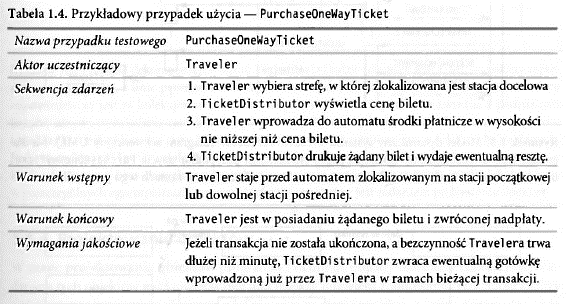
\includegraphics[width=14cm]{images/hyps/use-case.png}
	\caption{Źródło:  Inżynieria oprogramowania w ujęciu obiektowym. UML, wzorce projektowe i Java, Bernd Bruegge, Allen H. Dutoit}
\end{figure}

\subsection {Faza analizy}

Kolejną fazą jest faza analizy, w której przede wszystkim ustala się kto będzie używał tworzonego systemu, co dany system ma robić oraz kiedy i gdzie będzie używany. Na tym etapie powstaje model który jest wynikiem zgromadzenia wymagań klienta jak i również wyciągniętych wniosków z przeprowadzonych przypadków użycia ( z ang. Use Cases) Po zakończeniu tej fazy otrzymanym rezultatem jest model systemu wzbogacony o atrybuty operacji i skojarzenia, który jest spójny i wolny od niejednoznaczności. Ewentualne jego przejawy bądź niespójności modelu są omawiane podczas negocjacji z klientem.\\

\subsection {Faza projektowania}

W porównaniu do dwóch poprzednich etapów, w którym główny nacisk był nakładany na ideę stojącą za stworzeniem konkretnego projektu, tak w tym pojawia się po raz pierwszy kreowanie w jaki sposób ma to być zrealizowane. Tutaj powstają wstępne koncepcję wewnętrznej logiki działania projektu. Dochodzi do projektowania interfejsów między innymi interfejsu użytkownika, także dyskutowana jest architektura systemu. Zdarza się, że dochodzi do podziału na dwie mniejsze fazy: faza projektowania systemu oraz projektowanie obiektów.\\
\begin{itemize}
	\item  wybór platformy sprzętowej oraz systemu operacyjnego środowiska docelowego 
	\item selekcja technologii użytych i sposobu przechowywania danych tworzonego oprogramowania 
	\item podejmowane są również decyzję w sprawie globalnej kontroli przepływu sterowania oraz reguł polityki dostępu \\
\end{itemize}
Podobnie jak w poprzedniej fazie czyli fazie analizy rezultatem otrzymanym na koniec jest klarowny opis i reprezentacja budowanego systemu w postaci na przykład diagramu. Główną różnicą jest fakt, że otrzymane modele systemu nie są zrozumiałe dla klienta tak jak to było w fazie analizy. Są one bowiem stworzone za pomocą raczej zaawansowanych i ulepszonych technik, które przekraczają możliwości zrozumienia i zainteresowania przeciętnego klienta.\\
Wspomniana wcześniej faza projektowania obiektów ma na celu zasklepienie luk pomiędzy modelem zbudowanym podczas etapu analizy, a platformą sprzętową i programową zdefiniowaną na etapie projektowania systemu. Podczas tej fazy zostaje uszczegółowione oraz sprecyzowane opisanie poszczególnych obiektów i podsystemów w celu osiągnięcia rozszerzalności, zrozumienia oraz poprawy wydajności tworzonego systemu. Rezultatem tego etapu jest szczegółowy model obiektowy który posiada szeroko rozwinięte spektrum wyjaśniające wszystkie elementy.\\

\subsection {Faza implementacji}
Faza implementacji to w rzeczywistości wprowadzenie w życie wszystkich planów które zostały dotychczas stworzone. W żargonie programistycznym można powiedzieć, że jest to tłumaczenie modeli na kod źródłowy aplikacji. Oznacza to programowanie każdego obiektu zaprojektowanego w poprzednich etapach, a następnie zintegrowanie ich w jeden działający pojedynczy system. Rezultatem tego etapu jest zasklepienie przerwy pomiędzy skomplikowanymi i uszczegółowionymi diagramami, planami oraz modelami a skończonym i kompilowanym kodem źródłowym.\\

\subsection {Faza testowania}
Ostatnią fazą jest faza testów która wykonywana jest już na stworzonym w poprzednim etapie działającym systemie. Polega na analizie założonych zachowań i funkcjonalności podczas projektowania a jego rzeczywistym odwzorowaniem w gotowym oprogramowaniu. To w niej wykonywana jest zdecydowana większość testów, jednak niektóre z nich były już obecne w poprzedniej fazie. Biorąc pod uwagę ilość różnych poziomów testów, poniższa grupa jest najpopularniejszą, jeśli chodzi o zdecydowaną większość projektów informatycznych. Testy dzielone są na:\\

\begin{itemize}
	\item Testy jednostkowe
	\item Testy integracyjne
	\item Testy obciążeniowe
	\item Testy funkcjonalne
	\item Testy akceptacyjne \\
\end{itemize}

\subsubsection {Testy jednostkowe}
Testy jednostkowe to testy, których zadaniem jest sprawdzenie poprawności działania pojedynczego, wyizolowanego bytu. Są to najczęściej pojedyncze funkcję, jednostki bądź komponenty. Kluczową cechą tych testów jest brak integracji z API bądź bazą danych (jest to zadanie testów integracyjnych). Tego typu testy muszą działać bardzo szybko (liczone w setkach na sekundę), ponieważ odpalane są wiele razy przez programistów w fazie implementacji. Mają one nie tylko sprawdzać poprawność testowanego komponentu, ale przede wszystkim być dać deweloperom pewność siebie, że implementowane przez nich zmiany w kodzie nie doprowadzą do usterek funkcjonalnych. \\

\begin{figure}[h]
	\centering
	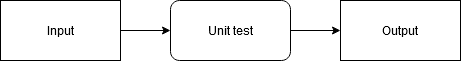
\includegraphics[width=12cm]{images/hyps/unit-test-flow.png}
	\caption{Uproszczony diagram działania testów jednostkowych}
\end{figure}

\subsubsection {Testy integracyjne}
Testy integracyjne są często łączone z testami jednostkowymi, ponieważ są one do siebie bardzo podobne. Diametralną różnicą jest fakt, że testy jednostkowe nie sprawdzają integralności między komponentami a API czy bazą danych, natomiast testy integracyjne już tak. Wykonywane są w celu wykrycia wad i defektów w interfejsach i komponentach oraz służą do testowania poprawnej interakcji między modułami lub systemami. Są one przeprowadzane w celu oceny zgodności systemu lub komponentów z określonymi wymaganiami funkcjonalnymi. Test integracyjny traktuje system jak czarną skrzynka. Testują integralność bez zagłębiania się w szczegóły implementacji, co oznacza, że otrzymywana jest tylko informacja, jaka konkretna funkcjonalność powinna działać oraz co zostać zwrócone jako wynik. Weryfikowane jest czy otrzymany rezultat zgadza się z oczekiwanym wynikiem bazującym na danych wejściowych. Podobnie jak testy jednostkowe są tutaj sprawdzone zaimplementowane funkcje oraz poprawność interfejsów, które powinny zapewnić integralność systemu, mogą one również wskazać błędy w strukturach danych bądź problemy z dostępem do API lub bazy danych.\\

\subsubsection {Testy obciążeniowe}
Testy obciążeniowe nazywane mogą być również testami wydajnościowymi ze względu na ich główny cel. Podczas ich wykonywania testowana jest próba obciążenia serwera, bazy danych oraz samego systemu naszej aplikacji bazując na wcześniej przygotowanych scenariuszach użycia oraz w oparciu o wygenerowane wirtualnych użytkowników których zadaniem jest wykonanie wcześniej stworzonych scenariuszy. Przykładowymi scenariuszami użycia są wszelkie działania, które może wykonać klient na przykład proces rejestracji czy logowania. Testy obciążeniowe mają za zadanie wskazać krytyczne punkty systemu, które w negatywny sposób wpływają na wydajność tworzonego systemu. Sprawdzają realny ruch na serwerze, który następnie pozwala na zdobycie punktu odniesienia oraz możliwości sprawdzenia czy nasz projekt spełnia wymogi wydajnościowe, brak wiedzy z tego zakresu może doprowadzić do braku akceptacji na wdrożenia.\\

\subsubsection {Testy funkcjonalne}
Testy funkcjonalne są to testy które opierają się na analizie specyfiki funkcjonalnej tworzonego oprogramowania, systemu bądź modułu. Są one najczęściej wykonywane przez osoby które nie miały styczności z zaimplementowanym kodem. Testerzy mają za zadanie poddanie próbie stworzony system bez znajomości jego budowy. Głównym zamysłem nie jest przetestowanie konstrukcji bądź architektury lecz jego założenia funkcjonalne, to znaczy mają wykryć błędy zaimplementowanych funkcjonalności, które zostały zawarte w dokumentacji.\\

\subsubsection {Testy akceptacyjne}
Testy akceptacyjne to inny gatunek testów, ponieważ nie skupiają się one na znalezieniu błędów czy pomyłek w implementacji systemu, mają one na celu potwierdzenie wykonania oprogramowania na odpowiednim poziomie. Służą do uzyskania formalnego potwierdzenia od klienta bądź osób zewnętrznych, że wykonany projekt spełnia kryteria jakościowe. Ważnym ich aspektem jest również weryfikacja czy nie brakuje założonych w dokumentacji funkcjonalności oraz czy procesy biznesowe przechodzą w prawidłowy sposób, taki aby zbudowały zaufanie wśród odbiorców. Następnym testowanym czynnikiem jest potwierdzenie czy aplikacja jest zgodna z dokumentacją. Testy akceptacyjne są ostatnim etapem weryfikowania poprawności zrealizowania systemu informatycznego, na jego podstawie menedżerowie odpowiedzialni za rozwój projektu podejmują decyzję o wdrożeniu do użytkowania produkcyjnego. \\ \\ \\ \\ \\ \\ \\ \\

\begin{figure}[h]
	\centering
	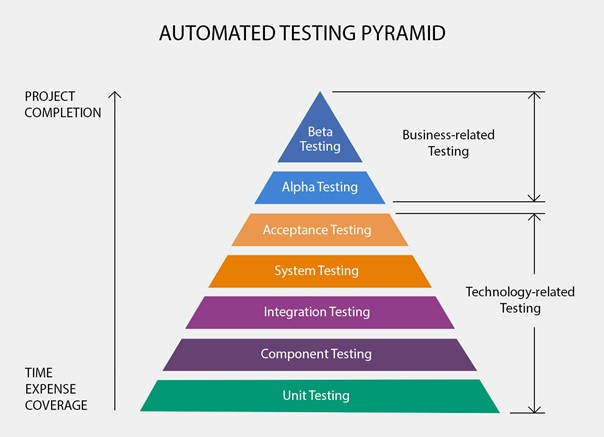
\includegraphics[width=15cm]{images/hyps/test-diagram.jpg}
	\caption{Piramida procesu przeprowadzania testów}
\end{figure}

\section {Metodyki w projekcie}
Pojęciem metodyki nazywamy zbiór metod służących do zarządzania projektem. Mówiąc prościej są to metody dzięki którym jest możliwe zakończenia projektu z powodzeniem w wyznaczonym czasie. Korzystanie z metodyki pozwala na uzyskanie maksymalnej wydajności podczas tworzenia oprogramowania. Chociaż metodyk jest sporo i wybór zależy stricte od charakterystyki projektu to w ramach uproszczenia można je podzielić na grupy.  Najogólniejszym i najpopularniejszym podziałem jest rozdzielenie na metodyki klasyczne (nazywane również tradycyjnymi) oraz zwinne. Do pierwszej grupy zaliczymy na przykład waterfall, natomiast do drugiej Agile.\\

\subsection {Podejście klasyczne a zwinne}
Aby umiejętnie wybrać odpowiednią metodykę do realizowanego projektu należy znać fundamentalne różnice między wcześniej wymienionymi grupami. \\

Metodyki klasyczne charakteryzują się wysokim stopniem planowania oraz uporządkowania. Projekty są podzielone na konkretne etapy a sam harmonogram prac oraz zakres i cel tworzonego projektu jest odgórnie znany. Natomiast metodyki zwinne uznawane są za zupełny kontrast metod tradycyjnych. Nie ma w nim konkretnego planu a praca przypomina swego rodzaju improwizacje dostosowywaną do zmienności okoliczności oraz ich losowości. Na ich podstawie ukazywane są nieznane wcześniej zakres i cel projektu. Są to kluczowe różnice pomiędzy tymi metodykami, stąd często są porównywane jako uporządkowane kontra elastyczne.\\

Kolejnym faktorem jest rozmiar projektu, w metodykach klasycznych tworzone są najczęściej duże i rozbudowane projekty. Wynika to z faktu że wielkie przedsięwzięcia wymagają, charakterystycznych dla podejść tradycyjnych, organizacji oraz planowania. Tak jak zostało to wcześniej wspomniane sukcesywne realizacje projektu bazującym na harmonogramie oraz celach poznanych na początku projektu. W mniejszych projektach rozmiar jak i czas przedsięwzięcia są najczęściej diametralnie mniejsze i krótsze. Nie wymagają tak ścisłych reguł działania oraz konsekwencji a co za tym idzie metodyki zwinne doskonale do nich pasują.\\

Kontakt z klientem w metodyce klasycznej nie jest konieczny. Występuje on na początku w fazie zbierania informacji oraz specyfikacji wymagań do projektu. Jak również na samym końcu przy prezentacji projektu. W charakterze zwinnym podejście jest ponownie odmienne, kontakt z klientem jest ciągły, stąd też wspomniana wcześniej tendencja do zmian w trakcie projektu, bowiem klienci zgłaszają swoje opinie oraz zastrzeżenia w trakcie realizacji projektu co często doprowadza do przekształcania zakresu projektu.\\

Zaangażowanie zasobów ludzkich w obu metodykach jest ponownie różne. W charakterystyce zwinnej nie ma ustalonej hierarchii pracowników, posiadają oni sporą autonomię a ich współpraca jest dostrzegalna na praktycznie wszystkich płaszczyznach. Sytuacja w metodyce tradycyjnej wprowadza hierarchię, w zespołach występuje osoba która nie wykonuje tych samych zadań co pozostali członkowie zespołu - lider.\\

Poniższa tabela w skondensowany sposób przedstawia kontrast między dwoma metodykami.\\

\begin{figure}[h]
	\centering
	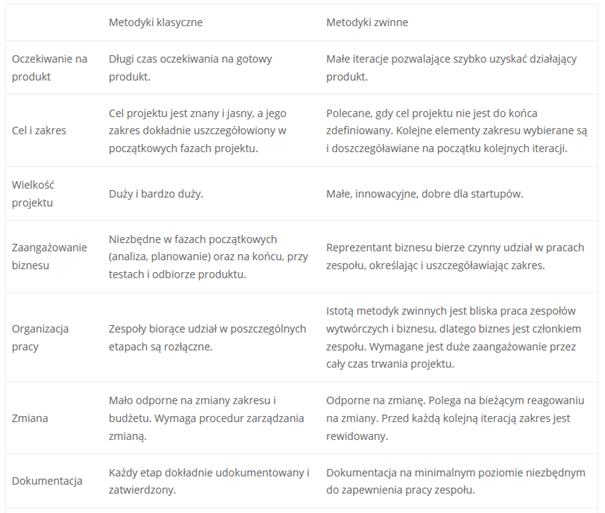
\includegraphics[width=15cm]{images/hyps/zwinne-tradycyjne.png}
	\caption{Źródło: Narudo, Zwinne i tradycyjne zarządzanie projektem}
\end{figure}

\subsection {Metoda waterfall}
Metoda waterfall to przykład modelu kaskadowego nazywanym również klasycznym, to jeden z wielu rodzajów procesów stworzenia oprogramowania. Polega na kaskadowym przechodzeniu pomiędzy ukończonymi wcześniej fazami. Zgodnie z wizją autora tej metodyki o sukcesie projektu decydują dokładne zaplanowanie poszczególnych zadań oraz bezwzględne przestrzeganie terminów. Najważniejszym elementem tej metody jest szczegółowy plan oraz tworzona dokumentacja do każdej fazy projektu. Zakłada on sekwencyjną realizacje ustalonych etapów. Występują one kolejno po sobie i tworzą niezależne zadania. W wyniku braku możliwości przejścia do następnego etapu przed zakończeniem poprzedniego występuje wysokie ryzyko pojawienia się błędów które będą bardzo kosztowne w naprawie.\\


\begin{figure}[h]
	\centering
	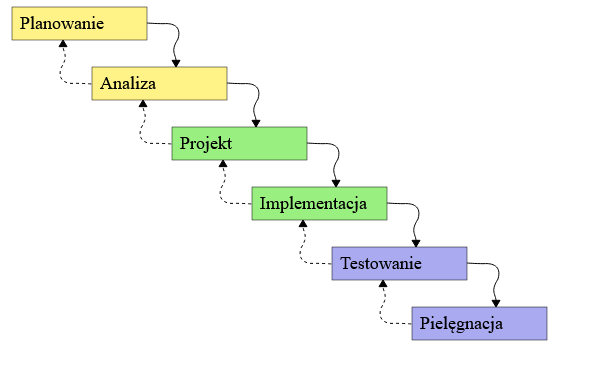
\includegraphics[width=15cm]{images/hyps/waterfall.png}
	\caption{Źródło: Wikipedia, Fazy modelu kaskadowego, Maciej Jaros - Praca własna}
\end{figure}

\subsection{Metody zwinne czyli Agile}

\subsubsection{Manifest Agile}
Manifest agile wprowadzony w 2001 roku zaproponował i wprowadził nowe spojrzenie na możliwości wytwarzania oprogramowania. Przede wszystkim podkreślił wagę pracy zespołowej i interakcji międzyludzkiej nad dotychczasowej koncentracji na procesach i narzędziach. Zwrócono uwagę nad kontaktem z klientem oraz na tworzeniu roboczego oprogramowania zamiast wszechstronnej dokumentacji. Największym przeciwieństwem do dotychczasowych metod było zaakceptowanie powrotu do fazy implementacyjnej w celu zareagowania na błędy i sugestie.\\ \\

\begin{figure}[h]
	\centering
	
\includegraphics[width=15cm]{images/hyps/manifest.png}
	\caption{Źródło: Agile247, Manifest zwinnego programowania}
\end{figure}

Generalnym założeniem stało się restrykcyjne zarządzanie procesem wytwarzania oprogramowania. Zakładana jest regularna kontrola wymagań jak i rozwiązań wraz z procesami adaptacji projektowych. Dużą wagę przywiązuje się do bezpośredniej komunikacji pomiędzy osobami z zespołu oraz codziennego kontaktu między sobą. W wyniku braku zastosowania jakiekolwiek hierarchii organizacyjnej na barkach członków zespołu spoczywa większy ciężar dbania o systematykę i organizację pracy. Odpowiedzialność ta spoczywa bezpośrednio na osobach realizujących poszczególne zadania.\\

\subsubsection{Czym jest model iteracyjny w Agile?}
Podejście zwinne jest grupą metod, które bazują na tworzeniu oprogramowania opartym na stylu iteracyjno-przerostowym. Głównym jego założeniem jest tworzenie i wdrażanie systemu etapami. Pojedyncza iteracja kończy zrealizowany cykl życia projektu etapem testów. Wówczas zrealizowana część zostanie przekazana odpowiedniej grupie odpowiedzialnej ze przeprowadzenie sprawdzenia poprawności działania. Testowana jest również praktyczność zastosowania podczas realizacji faktycznych założeń biznesowych. Zdobywanie regularnej informacji zwrotnej pozwala na cykliczne korekty błędów, wprowadzanie zmian i ulepszeń funkcjonalności oraz precyzyjne reakcje na potrzeby klienta. Stąd, jak wspomniane wcześniej tendencję do ewolucji funkcjonalności w projekcie. Pojedynczy cykl rozpoczyna się od fazy szczegółowego planowania zadań rozłożonych w konkretnym cyklu. Najczęściej przygotowywany jest przez szefów zespołów programistycznych lub kierowników projektowych. Następnym krokiem jest implementacja wcześniej przygotowanych założeń i funkcjonalności po której następuje czas na testy i wdrożenie. To tutaj docelowa grupa bada jakość przygotowanej cząstki projektowej i decyduje o możliwości wdrożenia oraz przejścia do kolejnej iteracji.\\

Poniższy model obrazuje podejście iteracyjne, które jest charakterystyczne w metodyce Agile. \\

\begin{figure}[h]
	\centering
	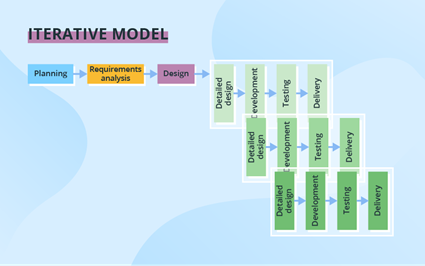
\includegraphics[width=15cm]{images/hyps/iterative-model.png}
	\caption{Źródło: ScienceSoft, Iterative model}
\end{figure}

\section{Wykorzystanie Agile w tworzeniu gry}
\subsection{Agile Game Development}
Agile Game Development to angielska nazwa na wykorzystanie podejścia zwinnego w tworzeniu gry komputerowej. Samo podejście nie różni się niczym szczególnym od standardowego. Kluczowe jest natomiast pokazanie jak wiele możliwości wprowadza Agile do życia projektu gry. Głównym z nim jest wcześniej rozwinięty model iteracyjny. Dzięki niemu cząstki gry, posiadające nowe funkcjonalności, znacznie częściej trafiają na testy do grupy docelowej. Takie podejście pozwoliło naprawić wiele błędów, których nie udało się wykryć w fazie implementacyjnej oraz poprawić działanie wielu funkcjonalności. Podczas realizacji zadań i rozwijania gry, programista może wpaść w pułapkę subiektywnej opinii dotyczącej zaimplementowanych rozwiązań. Jak to zwykle się zdarza bywają one błędne i posiadanie możliwości weryfikacji tego na tak wstępnym etapie wprowadza ogromną wartość w projekcie. Pomimo przypisaniu takich elementów jak model iteracyjny czy częsty kontakt z klientem do podejścia zwinnego to w rzeczywistości są to nadrzędne składowe metod, z których składa się metodyka Agile (przypominając metodyka to zbiór wcześniej założonych metod). W projekcie „The Lore” została wykorzystana fuzja trzech najpopularniejszych, ponieważ jest to najbardziej znana i wykorzystywana strategia w projektach komercyjnych. Do tej grupy należą:\\

\begin{itemize}
	\item SCRUM
	\item Kanban
	\item XP - Programowanie Ekstremalne \\
\end{itemize}

\subsubsection{SCRUM}

Scrum to zdecydowanie kluczowa i prawdopodobnie najważniejsza część Agile. To ona jest odpowiedzialna za zarządzanie procesem iteracyjnym w projekcie. Jednak w tym przypadku pojedyncze iteracje nazywane są sprintami. Czyli wcześniej zdefiniowanymi partiami pracy, posiadającymi przypisane do nich zadania do wykonania oraz z wydzielonym terminem. Sprinty trwają najczęściej od dwóch do czterech tygodni w zależności od zarządzeń czy planów biznesowych. W przypadku „The Lore” sprinty w początkowej fazie prac, czyli około trzech miesięcy trwały dwa tygodnie, a następnie zostało to zredukowane do jednego tygodnia. Wynikało to z wzrostu jakości otrzymywanego produktu, ponieważ był on częściej oddawany w ręce testerów, a także sam proces programistyczny mógł być lepiej rozplanowany. Dawało to możliwość przypisania sprintów do wykonania konkretnych funkcjonalności zamiast tworzenia przeładowanego sprintu z różnymi funkcjonalnościami. Tym samym wzrosła wydajność pracy, ponieważ grupa docelowa oczekiwała już gotowego uaktualnienia produktu. Kolejnym doskonałym elementem scrum’u jest wprowadzenie ról poszczególnych członków zespołu. Jak wcześniej było wspomniane w podejściu zwinnym brakuje hierarchizacji w zespole co może doprowadzić do katastrofy organizacyjnej. Dlatego też Scrum wprowadza trzy funkcje:

\begin{itemize}
	\item Scrum Master
	\item Właściciel produktu
	\item Zespół deweloperski \\
\end{itemize}

Scrum master to przede wszystkim osoba odpowiedzialna za pilnowanie przestrzegania zasad Scrumowych. Diametralnie wpłynął na wydajność i produktywność zespołu, ponieważ wielokrotnie podczas sprintów pilnował postępów prac oraz jakości ich wykonania. Zajmował się również komunikacją z źródłami zewnętrznymi po to aby pozostałe osoby z zespołu nie musiały tracić na to czasu i odrywać się od pracy. Do jego obowiązków należało również planowanie szczególnych spotkań, tak zwanych retrospektyw oraz przeglądów sprintów. \\

Retrospektywą nazywamy spotkaniem odbywającym się cyklicznie co 2-3 tygodnie w celu ustalenia organizacji pracy, dyskusji o odczuciach każdego członka zespołu na poszczególne tematy. Czasami bywały to rozmowy stricte związane z kodem, jednak bywały też takie, które dotyczyły jakości pracy bądź kontaktami interpersonalnymi. W dużym uproszczeniu jest to czas dla zespołu aby mógł przedyskutować to co się podoba, nie podoba i jakie można podjąć akcję aby to zmienić. \\

Przegląd sprintu jest również cyklicznym spotkaniem, jednak odbywał się częściej – po każdym zakończonym sprincie. Jego głównym zadaniem jest dyskusja członków zespołu o stworzonych przez nich funkcjonalnościach. Dzielona jest wiedza w jaki sposób konkretny deweloper podszedł do wykonania zadania oraz w jaki sposób go zrealizował. Dzięki temu w sytuacji gdy inna osoba z zespołu otrzymała zadanie rozwoju tej funkcjonalności, w kolejnym sprincie, miała ona już bazę wiedzy wystarczającą do jego realizacji. Pozwala to na zaoszczędzenie czasu potrzebnego do zrozumienia działania kodu napisanego przez inne osoby. Podczas przeglądu sprintów tworzony jest również następny sprint, w którego skład wchodzą zadania bazujące na tworzeniu funkcjonalności zgodnie z harmonogramem. Po wypełnieniu nowego sprintu konkretnymi zadaniami, dochodziło do rozmowy o przydziale ich do konkretnej osoby. Głównymi czynnikami doboru zadań do członków zespołu było ich doświadczenie pracy z zadaniami łączonymi bądź zależnymi, które były wykonane w wcześniejszych sprintach. \\

Właścicielem produktu jest najczęściej osoba, poza zespołem, zlecająca wykonanie projektu, jednak w przypadku gry „The Lore”, ten tytuł spoczywał na barkach członka zespołu. Jego zadaniem było zadbanie o klarowną wizję projektu i pilnowanie czy tworzony projekt jest zgodnie z nią realizowany. Odpowiadał również za rozwój jak i maksymalizacje wartości produktu. Robił to przy użyciu decydowania o kolejności wykonywania prac i wprowadzanych funkcjonalności. Zarządzał również ich priorytetem i decydował o treści tworzonych zadań. Wykonywał to wraz z Scrum Masterem, jednak to jego decyzja była najważniejsza. Projekt był tworzony i rozpisany zgodnie z jego wizją produktu finalnego.\\

Ostatnią grupą jest zespół deweloperski. Charakterystyką tej roli jest odpowiedzialność za dostarczenie, przygotowanej przez nich, gotowej do wydania aktualizacji projektu. Realizują backlog sprintu, przygotowanego wcześniej podczas przeglądu sprintów.

\begin{figure}[h]
	\centering
	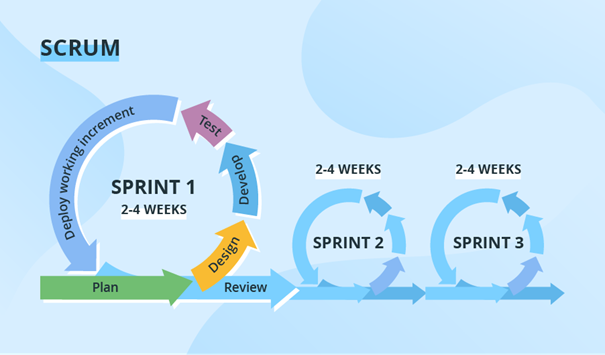
\includegraphics[width=13cm]{images/hyps/scrum.png}
	\caption{Źródło: ScienceSoft, SCRUM}
\end{figure}

Na powyższym zdjęciu prezentowany jest cykl realizacji sprintów oraz poglądowa wizaulizacja modelu pracy w Scrum'ie. \\ 

\subsubsection{Kanban}
Kanban to kolejna metoda w metodyce Agile. Jej głównym założeniem jest wizualizacja procesu realizacji zadań. Przy użyciu tak zwanej tablicy kanbanowej było obrazowane w którym etapie znajduje się poszczególne zadanie. W projekcie „The Lore” tablica została podzielona na najprostszy układ tj. podział na czynności „do zrobienia”, „w trakcie realizacji” i  „zrobione”. Jej celem było doprowadzanie do sytuacji w której organizacja pracy poszczególnych osób z zespołu jest widoczna dla wszystkich. Dzięki temu proces realizacji zadań od siebie zależnych przechodził w procesie bezproblemowym i jawnym. Jednocześnie dawało to wizualne potwierdzenie na jakim etapie pracy jest każdy członek zespołu. Przy niezadowalającym tempie pracy interweniował Scrum master lub właściciel produktu.\\


\begin{figure}[h]
	\centering
	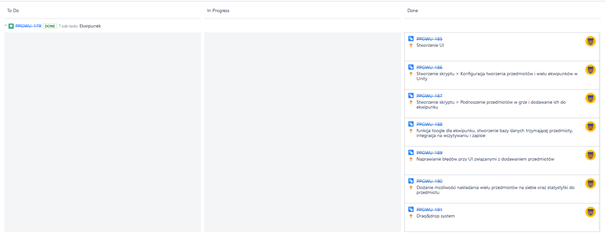
\includegraphics[width=15cm]{images/hyps/jira.png}
	\caption{Tablica kanbanowa w programie Jira. Przykład z projektu The Lore}
\end{figure}

„Jira to platforma do organizowania pracy i uruchamiania oraz monitoringu procesów w organizacjach.”  \cite{jira} Pozwala na utworzenie i zarządznie tablicą kanbanową w projektach.

\subsubsection{Programowanie ekstremalne}

Programowanie ekstremalne to już ostatnia metoda użyta w realizacji projektu „The Lore”, skupia się ona na adaptacji do częstych zmian wynikających z cyklicznych aktualizacji projektu. Głównym jego założeniem, który został wykorzystany jest „Pair programming” czyli programowanie w parze lub nawet większej grupie ludzi. Dzięki wspólnemu planowaniu, dyskutowaniu o potencjalnym rozwiązaniu, a następnie zaimplementowaniu go, maleje czas wykonania zadania które normalnie byłoby tworzone przez pojedynczego dewelopera. Szczególnie użyteczne gdy zbliża się termin zakończenia sprintu a zadanie jest w wczesnej fazie robienia lub gdy deweloper natrafił na „ślepy zaułek” i potrzebuje świeżego spojrzenia na zadanie. \\

\subsection{Cykl życia projektu The Lore}

\subsubsection{Faza zbierania informacji i analizy}

Podczas pierwszych faz realizacji projektu „The Lore” była tworzona szeroka dokumentacja, której zadaniem było zebranie jak najwięcej informacji potrzebnych do obrania odpowiedniego kierunku prac. Dzięki niej właściciel produktu wraz z scrum masterem mieli potencjalną wizję na tworzony harmonogram wraz z przygotowaniem backlogu z zadaniami na najbliższe sprinty. Dokumentacja wraz z później przygotowanymi na jej podstawie user stories była w tej fazie kluczowa. W skład dokumentacji wchodziła wizja projektu, VPC oraz BMC.\\

Dokument wizji projektu - jego głównym założeniem jest przedstawienie przeznaczenia tworzonego oprogramowania oraz jego głównych cech i przyjętych założeń. Dokument dzieli się na sekcje wprowadzenia, celu projektu, badania rynku, użytkowników docelowych, szczegółowego opisu produktu wraz z zakresem i ograniczeniami. \\

Value Proposition Canvas (VPC) to angielska nazwa na przedstawienie unikalnej propozycji wartości modelu biznesowego. Jego celem jest łatwiejsza analiza i zaprojektowanie  produktu wraz z jak najtrafniejszym skonfigurowaniem rozwiązań pod potrzeby klientów.\\ \\ \\ \\ \\ \\ \\

\begin{figure}[h]
	\centering
	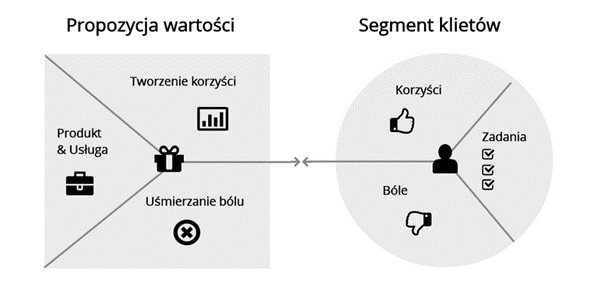
\includegraphics[width=10cm]{images/hyps/VPC.png}
	\caption{Źródło: Product Vision, Value Proposition Canvas}
\end{figure}

\begin{figure}[h]
	\centering
	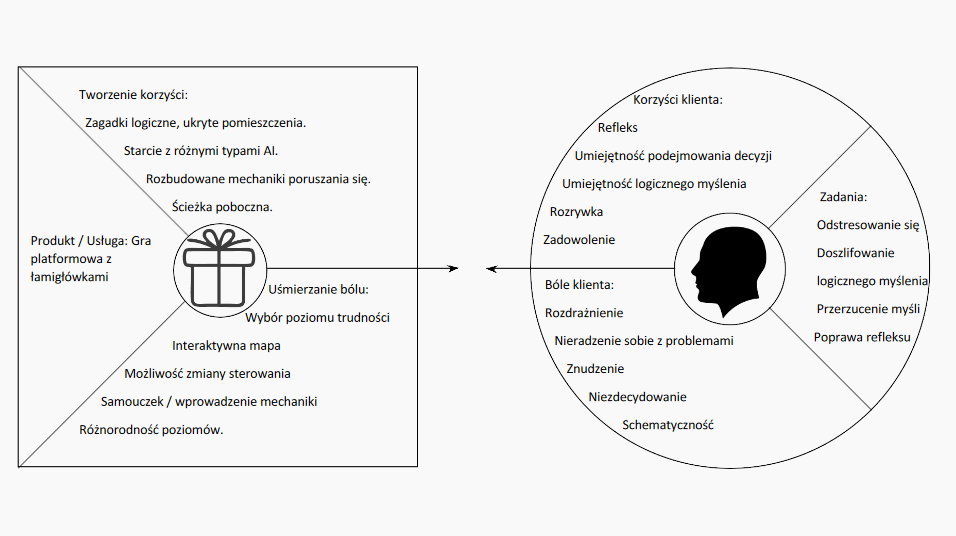
\includegraphics[width=11cm]{images/hyps/VPC-The Lore.png}
	\caption{Value Proposition Canvas dla projektu The Lore. Przykład z The Lore}
\end{figure}

Powyżej przedstawiony jest przykład unikalnej propozycji wartości modelu biznesowego oraz już oficjalny model z projektu gry "The Lore".\\ \\ \\ \\ \\ \\ \\ \\ \\ 

Business Model Canvas (BMC) to podobnie jak VPC angielska nazwa na szablon modelu biznesowego. Jego zadaniem jest w wizualny sposób przedstawienie w jaki sposób planowany projekt ma przynieść zyski. Składa się z 9 podstawowych obszarów, które obrazują grupę docelowych użytkowników oraz w jaki sposób zostanie im dostarczony produkt. Jednocześnie pokazuje wszelkie korelacje z wydatkami jak i potencjalnymi zarobkami planowanego projektu.\\


\begin{figure}[h]
	\centering
	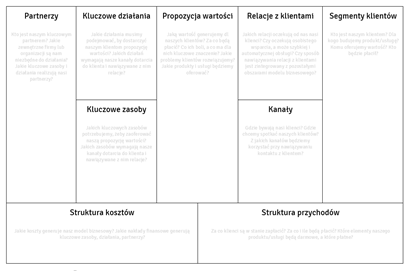
\includegraphics[width=15cm]{images/hyps/BMC.png}
	\caption{Źródło: Product Vision, Business Model Canvas}
\end{figure}

Powyżej przedstawiony jest przykładowy szablon modelu biznesowego. Natomiast poniżej już oficjalny model z projektu gry "The Lore".\\ \\ \\ \\ \\ \\ \\ \\ \\

\begin{figure}[h]
	\centering
	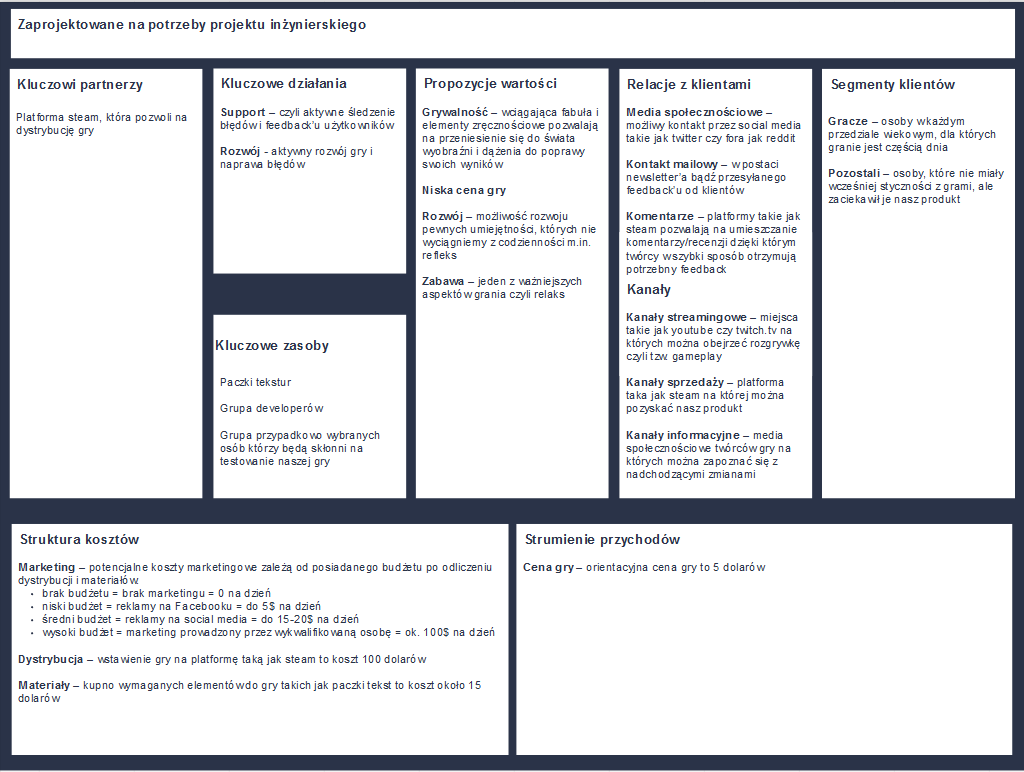
\includegraphics[width=10cm]{images/hyps/BMC - The Lore.png}
	\caption{Business Model Canvas dla projektu The Lore. Przykład z The Lore}
\end{figure}

\begin{figure}[h]
	\centering
	
\includegraphics[width=11cm]{images/hyps/backlog.png}
	\caption{Backlog z zadaniami w programie Jira. Przykład z The Lore}
\end{figure}

Utworzone user stories zostały wykorzystane do stworzenia pierwych zadań w backlogu projektu.\\ 

\subsubsection{Faza projektowania}

Po zakończeniu dwóch poprzednich faz w których rozwijany był zamysł stworzenia gry komputerowej „The Lore” przyszedł czas na skupienie się na tym w jaki sposób zostanie ona stworzona. Pierwszą rozterką było wybranie odpowiedniego środowiska. Pośród wielu możliwości na rynku, wybór padł na UNITY [wstawić załącznik do tego czym jest unity w technologiach]. Miał on opinię najbardziej przyjaznego dla początkujących twórców gier komputerowych. Posiadał on również najlepiej rozwiniętą dokumentację techniczną i największą bazę użytkowników udzielających się na specjalistycznych forach. Unity posiada również autorski sklep z materiałami, które są nieocenione przy tworzeniu gry w ograniczonym czasie. Po wybraniu środowiska trzeba było podjąć decyzję w sprawie używanego języka programowania. Tutaj jednak nie było to trudne, ponieważ z grupy Boo, UnityScript oraz C\# tylko ten ostatni był nadal wspierany przez Unity oraz cieszył się największą popularnością wśród twórców. Również był to najlepiej znany język w grupie deweloperskiej. Następnym etapem był wybór docelowej technologii oraz systemów na jakie ma trafić wdrożony projekt. Estymowany był tutaj dostępny czas oraz wymagania jakie kryją się za tworzeniem gry jednocześnie na urządzenia mobilne, stacjonarne jak i konsole. Niezależnie od możliwości jakie posiada Unity dla budowania projektu na różne platformy, sama implementacja funkcjonalności stwarzała komplikacje. Wynikały one z unikalnych cech każdej platformy. Stąd decyzja o wykonaniu gry na pojedynczą platformę – stacjonarną, ale z kompatybilnością na trzy najpopularniejsze systemy operacyjne – Windows, Linux, MacOS. Kolejnym etapem projektowania technicznego było dobranie odpowiedniej platformy wdrożeniowej. Na rynku jest ich dość sporo. Często różnice są marginalne i zależą od różnych twórców oraz cen za wdrożenie autorskiego projektu. Dylematem było wykorzystanie drogiego lecz jednocześnie najpopularniejszego miejsca na dystrybucję gry bądź wykorzystanie mało znanych platform, które udostępniają możliwość wdrożenia produktu za darmo. W związku z mocno ograniczonym budżetem projektowym, wybór musiał paść na platformę mniej znaną. Następnym elementem, który musiał zostać wybrany była platforma przechowywania plików. Tworząc projekt w pojedynkę, takie miejsce służy do bezpiecznego przechowywania progresu prac. Jednak przy pracy w zespole, tego typu miejsce służy również do współdzielenia i szybkiego dostępu do plików projektu. Najpopularniejszym na rynku środowiskiem jest Github. Wymagał on jednak specjalnej konfiguracji, ponieważ pliki przekazywane przez Unity są odmienne od standardowych. Przede wszystkim sam edytor Unity tworzy setki tymczasowych plików, które nie zawsze powinny trafić na Githuba. Odpowiednia konfiguracja pliku gitignore, którego celem jest nie przesyłanie wpisanych tam rozszerzeń, typów plików czy folderów była kluczowa. Kolejnym problemem z którym trzeba było sobie poradzić były błędne referencje do specjalistycznych obiektów w Unity. Tego typu informację wysyłane były na Githuba w specjalnych plikach z rozszerzeniem .meta, które rozwiązały wszelkie problemy z znikającymi obiektami stworzonymi przez programistów. Ostatnim i raczej największym problemem była konfliktowość wynikająca z edycji tych samych plików binarnych przez wielu programistów. Rozwiązanie ich podczas prób mergu branchy było niemożliwe. Stąd kluczowa była komunikacja wewnątrz zespołowa wraz z odpowiednią organizacją pracy i umiejętnym podziałem zadań. W fazie projektowania zostały tworzone również pierwsze szkice interfejsów graficznych. Wiele z nich zostało zmodyfikowanych lub zupełnie zmienionych.\\
Poniżej przedstawione są zdjęcia prototypów interfejsów graficznych głównego menu oraz menu sterowania.\\

\begin{figure}[h]
	\centering
	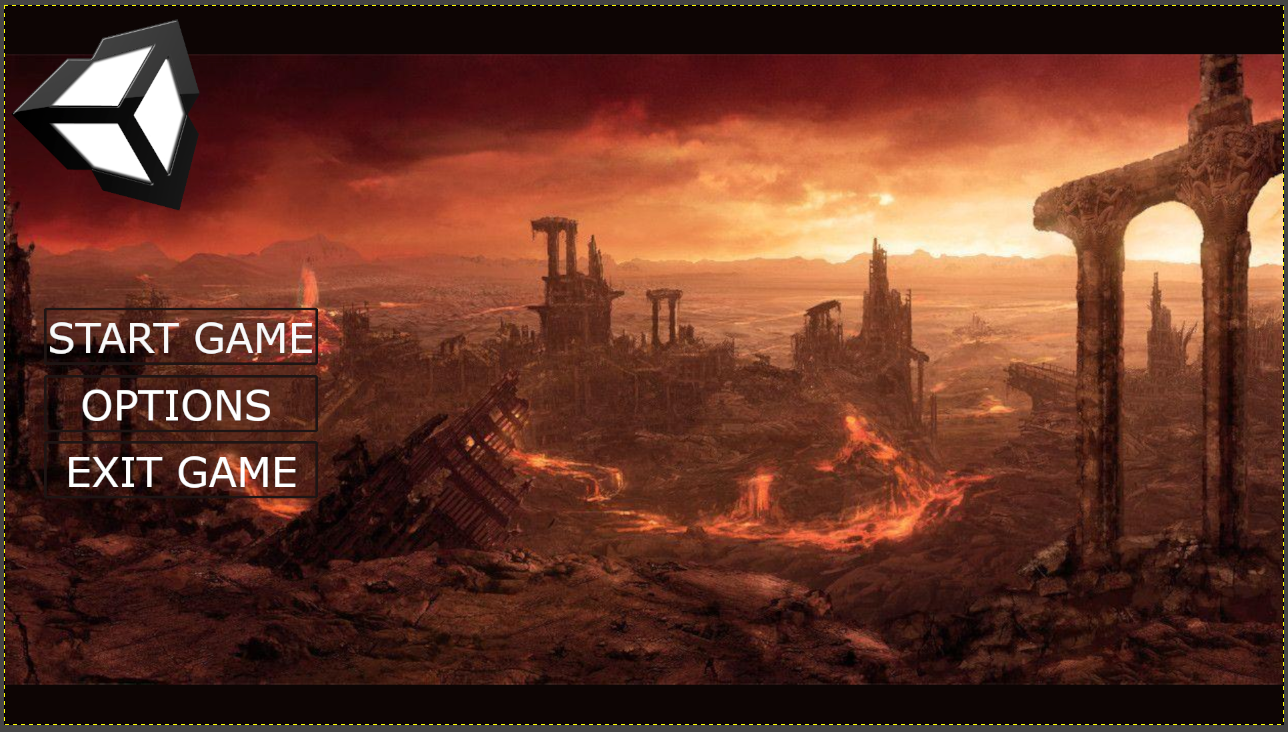
\includegraphics[width=12cm]{images/hyps/proto.png}
	\caption{Prototyp interfejsu menu głównego. Przykład z The Lore}
\end{figure}

\begin{figure}[h]
	\centering
	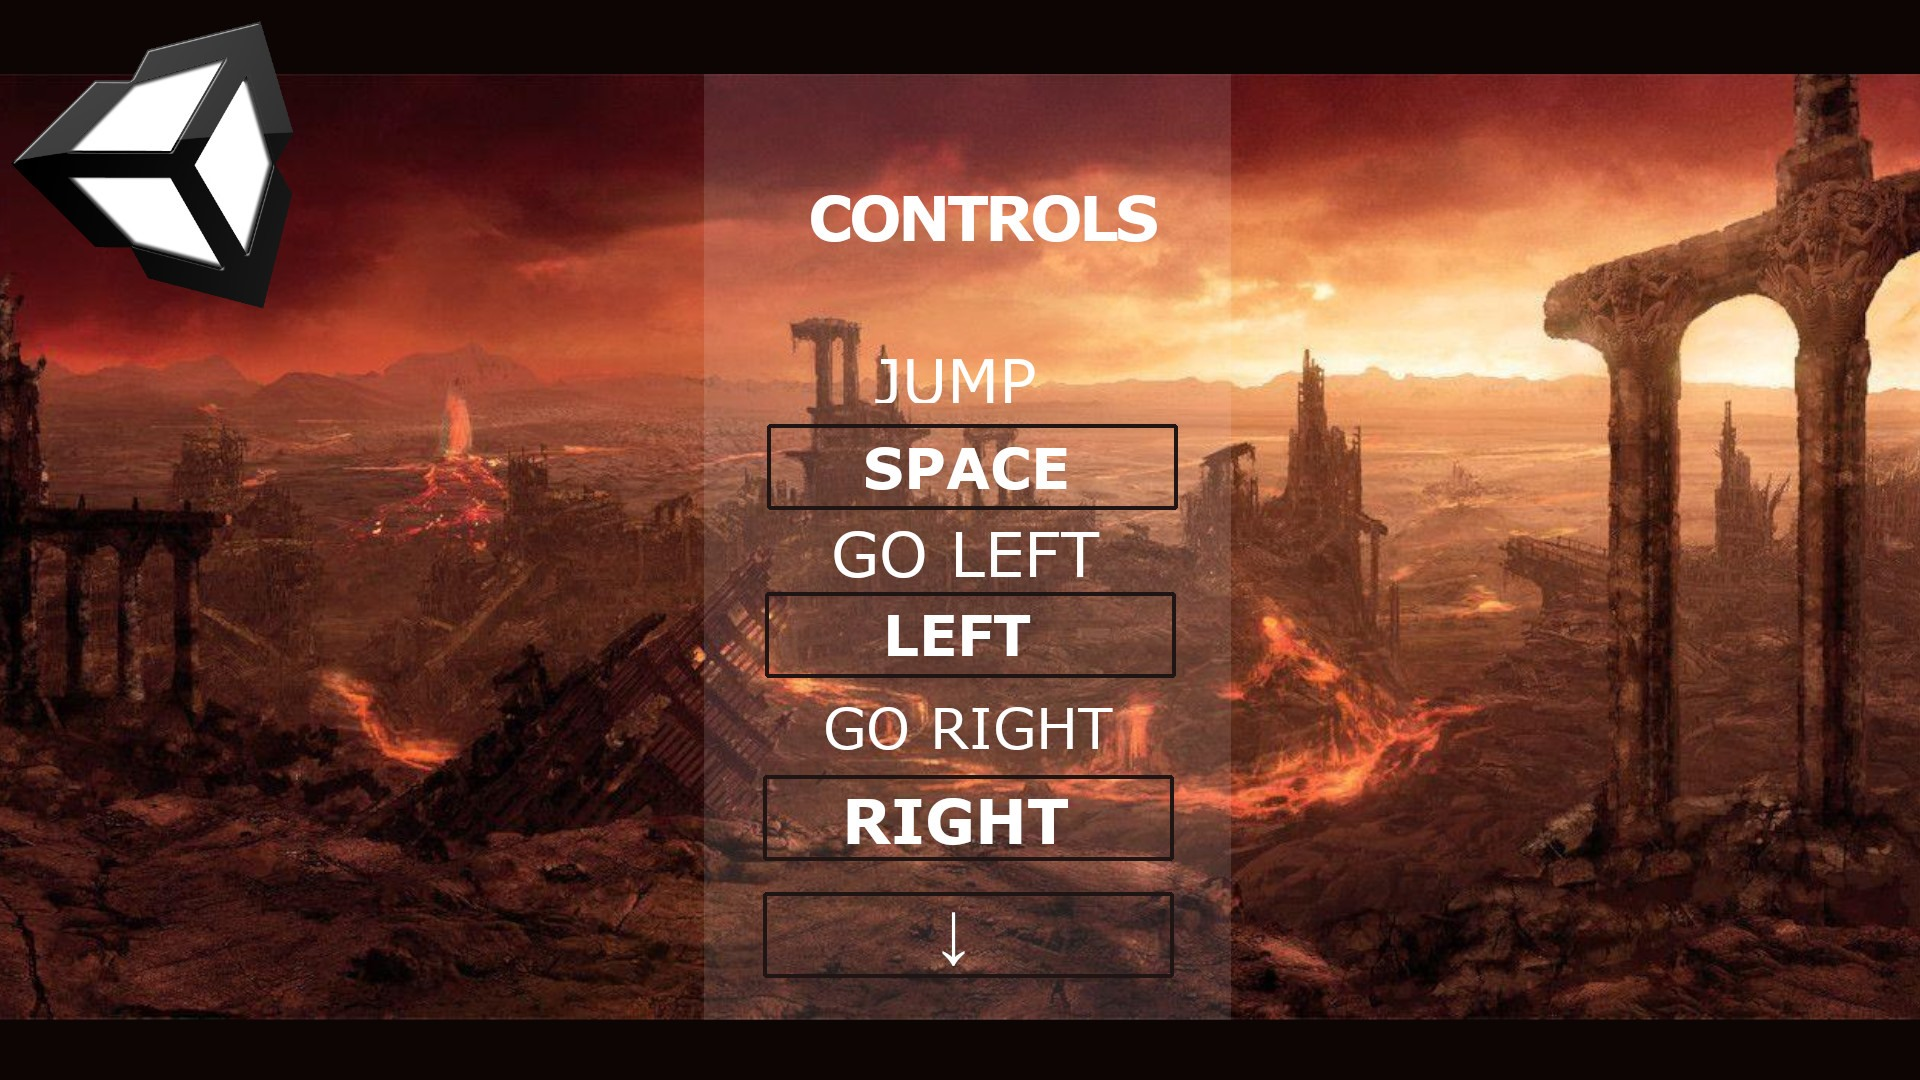
\includegraphics[width=12cm]{images/hyps/proto2.jpg}
	\caption{Prototyp interfejsu menu sterowania. Przykład z The Lore}
\end{figure}

Poniżej przedstawione są zdjęcia wdrożonych interfejsów graficznych głównego menu oraz menu sterowania.\\

\begin{figure}[h]
	\centering
	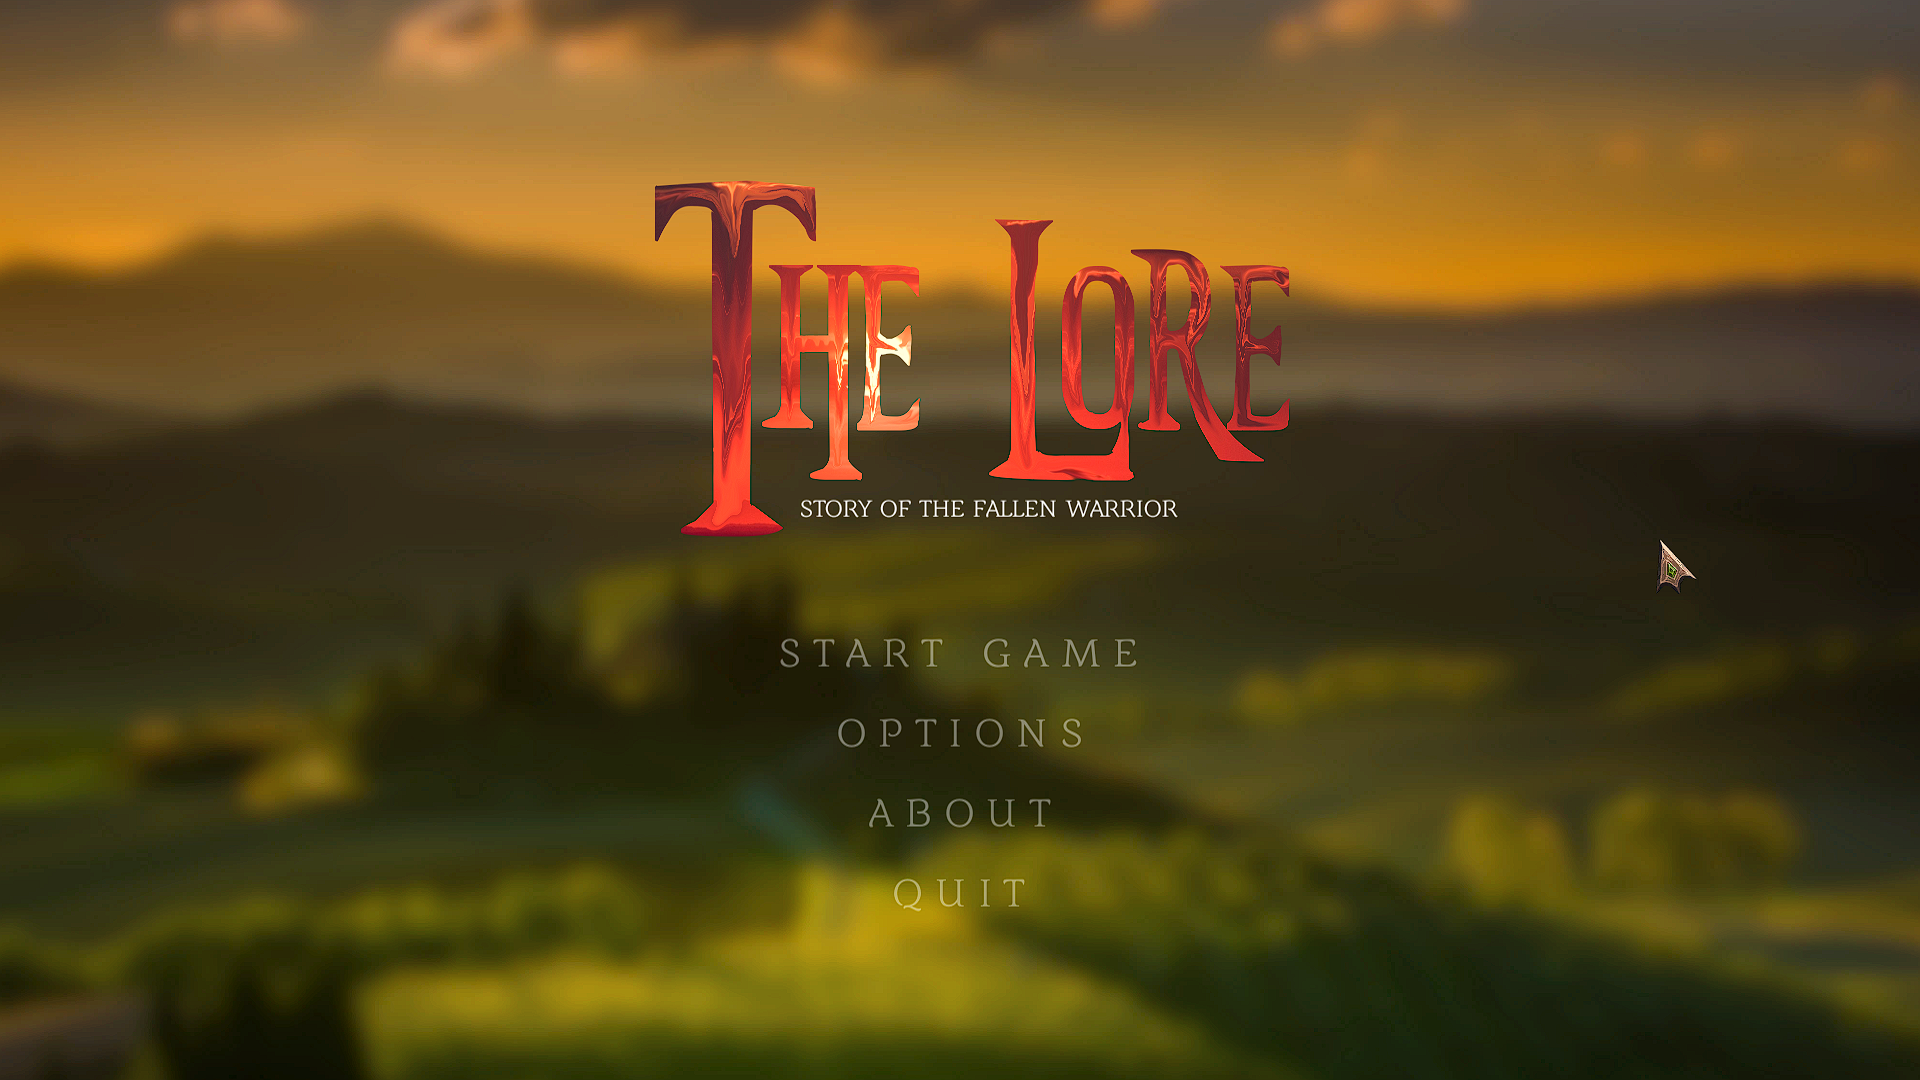
\includegraphics[width=12cm]{images/hyps/of1.png}
	\caption{Wdrożony interfejs menu głównego. Przykład z The Lore}
\end{figure}

\begin{figure}[h]
	\centering
	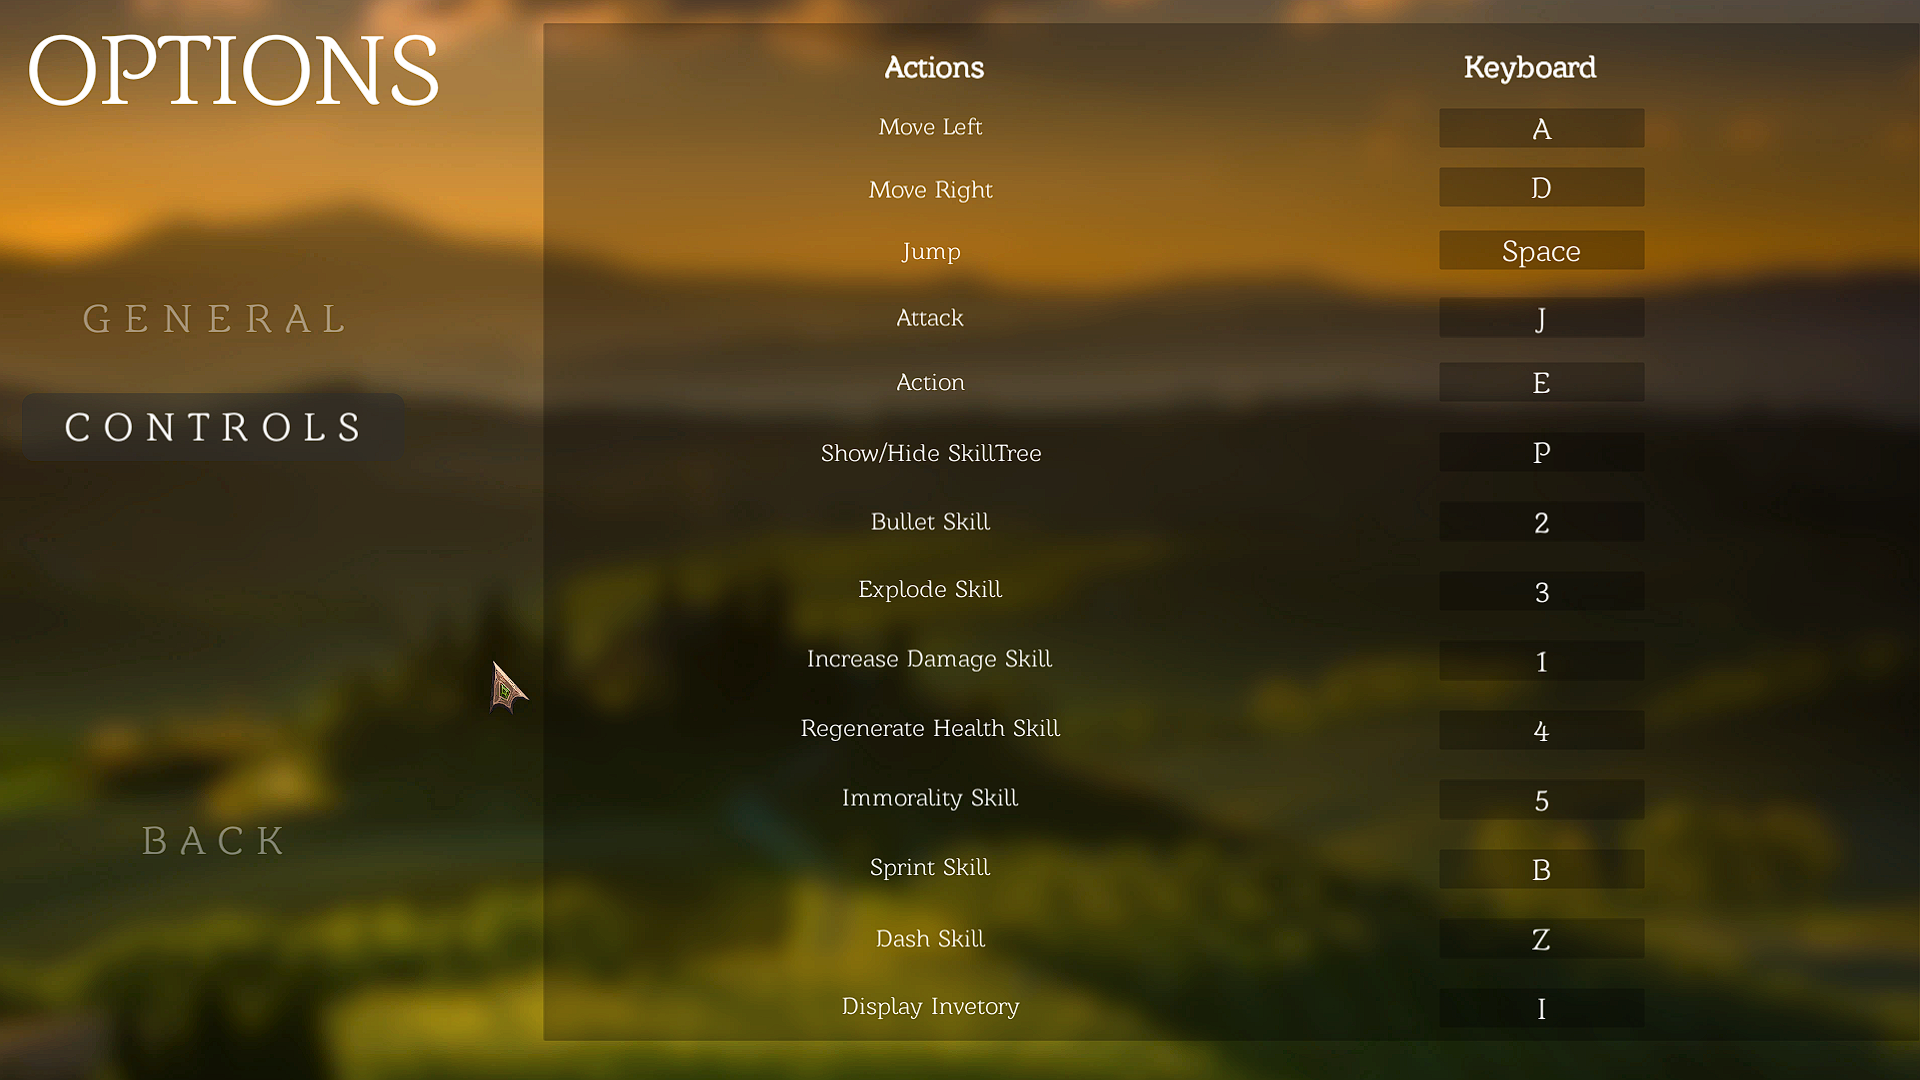
\includegraphics[width=12cm]{images/hyps/of2.png}
	\caption{Wdrożony interfejs menu sterowania. Przykład z The Lore}
\end{figure}

\subsubsection{Faza implementacji i testów}

Faza implementacji wraz z testami była powtarzana wielokrotnie w wyniku metodyki Agile. Poprzez model iteracyjny każdy sprint wykorzystywany był do zaimplementowania wcześniej zaprojektowanych funkcjonalności oraz przedstawienia ich grupie testerów. Dzięki nim w projekcie gry „The Lore” zespół deweloperski był w stanie na bieżąco wprowadzać wszelkie poprawki wraz z sugestiami otrzymywanymi podczas testów. Przykładową funkcjonalnością jest element poziomu samouczka – poruszające się platformy. Zgodnie z powtarzającą się opinią o trudności w przechodzeniu tego elementu, zostały wprowadzone poprawki wraz z dodatkowymi ułatwieniami. Przykładowym rozwiązaniem było dodanie specjalistycznej fizyki, która miała na celu przyciąganie gracza w kierunku nadchodzącej platformy. Innym, bardziej wizualnym ułatwieniem było dodanie tras po których poruszają się platformy. Ostatnim ułatwieniem było zmniejszenie prędkości poruszania się platform oraz powiększenie ich powierzchni. \\ \\ 
Poniżej przedstawiono zdjęcie z pierwszej iteracji tworzonej funkcjonalności\\

\begin{figure}[h]
	\centering
	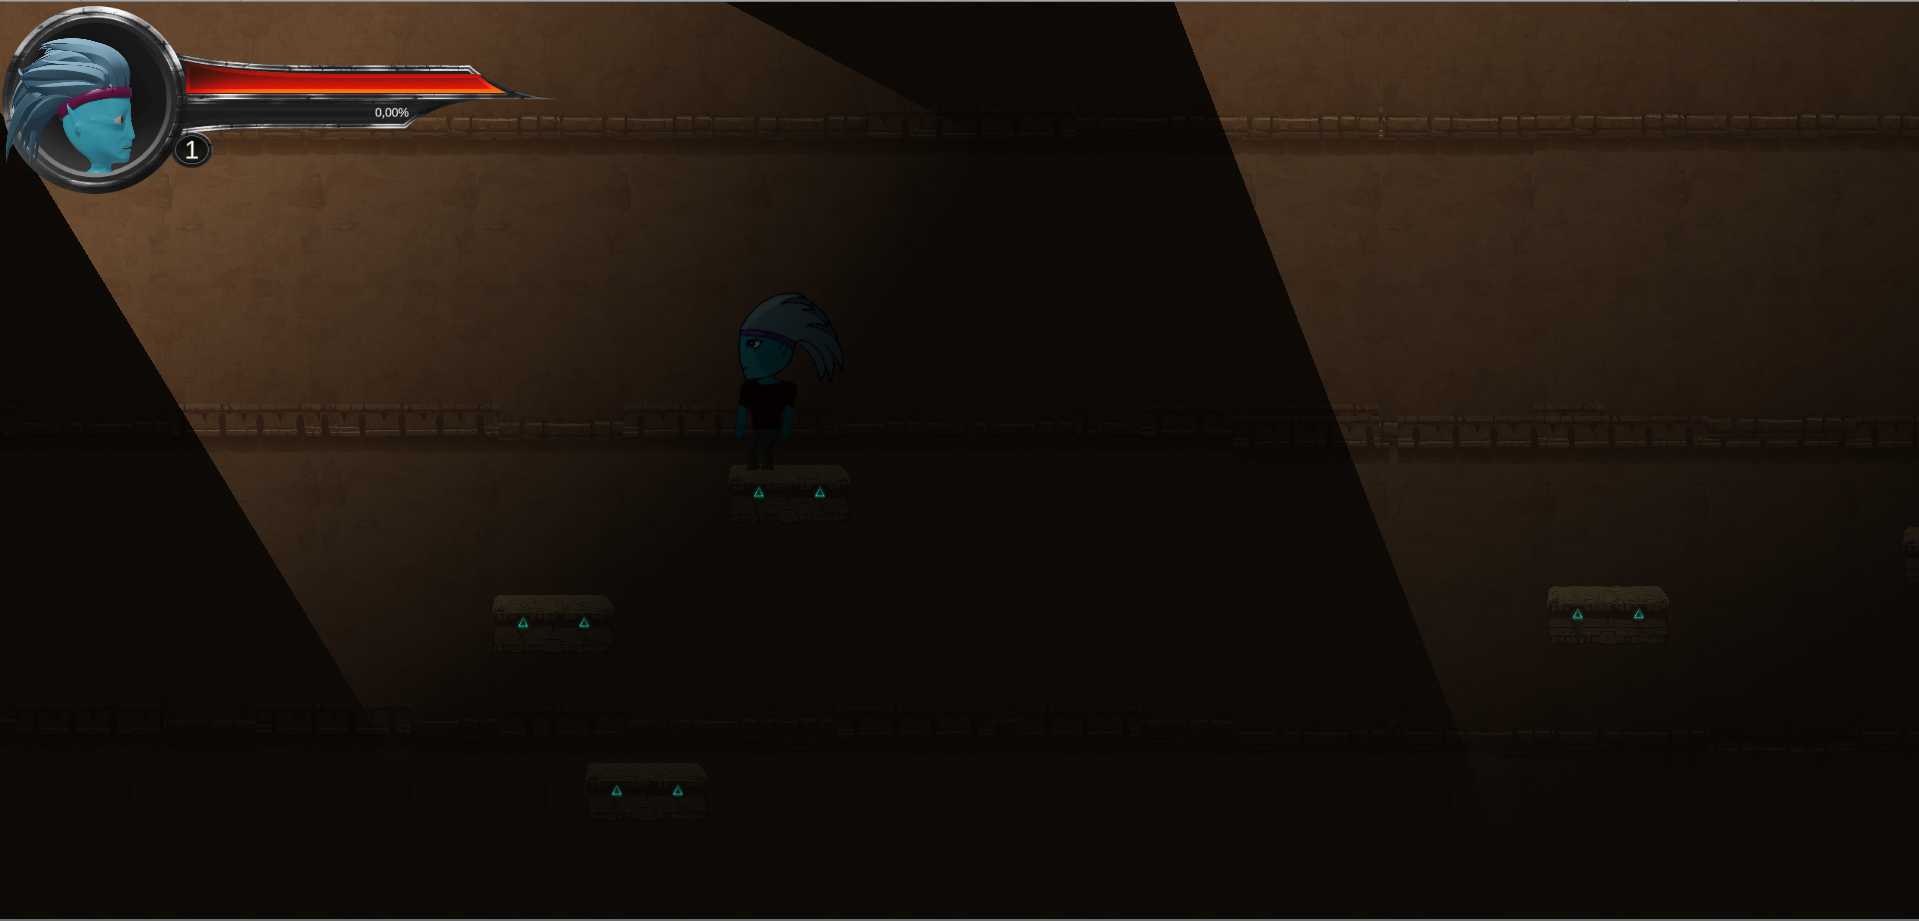
\includegraphics[width=14cm]{images/hyps/platfBef.png}
	\caption{Pierwsza iteracja ruchomych platform. Przykład z The Lore}
\end{figure}

Poniżej pokazana jest już ostania iteracja, która posiada wszelkie uwagi otrzymane z fazy testów \\ \\ \\ \\ \\ \\ \\ \\ \\ \\ \\

\begin{figure}[h]
	\centering
	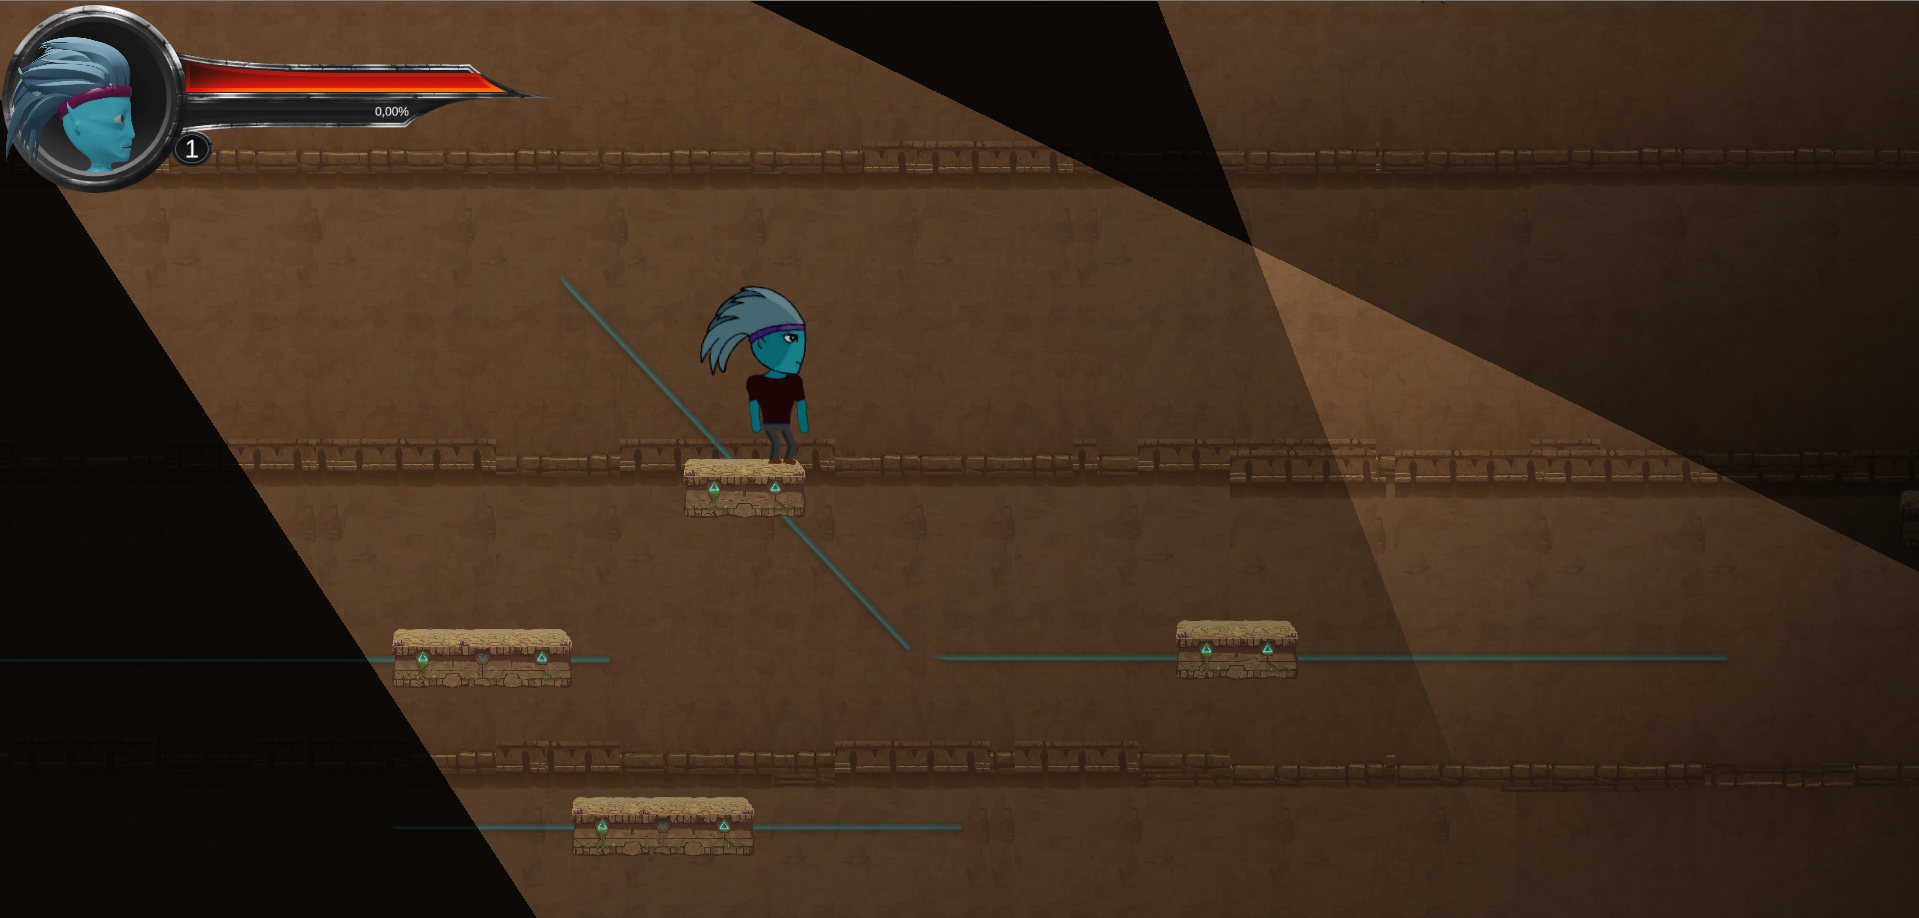
\includegraphics[width=14cm]{images/hyps/platfAfter.png}
	\caption{Ostatnia iteracja ruchomych platform. Przykład z The Lore}
\end{figure}

To był jeden z wielu procesów poprawionych dzięki otrzymanej opinii podczas testów, jednak wystarczająco poważny żeby pokazać jak kluczowym było wybranie metodyki Agile w projekcie stworzenia gry komputerowej „The Lore”.\\






\chapter{Zagadki logiczne}
\section{Wprowadzenie do zagadek logicznych}
\subsection{Omówienie zagadnienia}
Zagadką logiczną określamy zadanie, którego celem jest odnalezienie odpowiedzi na pytanie, logiczne dojście do rozwiązania problemu czy też czasami abstrakcyjne myślenie. Możemy wyróżnić różne rodzaje zagadek, między innymi graficzne, czego przykładem jest znany, często używany w szkołach podstawowych rebus. Główną ideą takiej rozgrywki jest rozwój swoich intelektualnych możliwości przy dobrej zabawie. \cite{zagadka_logiczna}
\subsection{Przykłady logicznych zagadek w prawdziwym świecie}
\subsubsection{Rebus}
Przywołanym już przykładem zagadki może być rebus. To prosta rozgrywka, polegająca na odgadnięciu hasła na podstawie przytoczonego obrazka. Często treści w rebusach mogą być niejednoznaczne, co sprawia, iż nie są one trywialne i wymagają wielu kombinacji haseł, związanych z danym obrazkiem. \cite{rebus}
\begin{figure}[h]
	\centering
	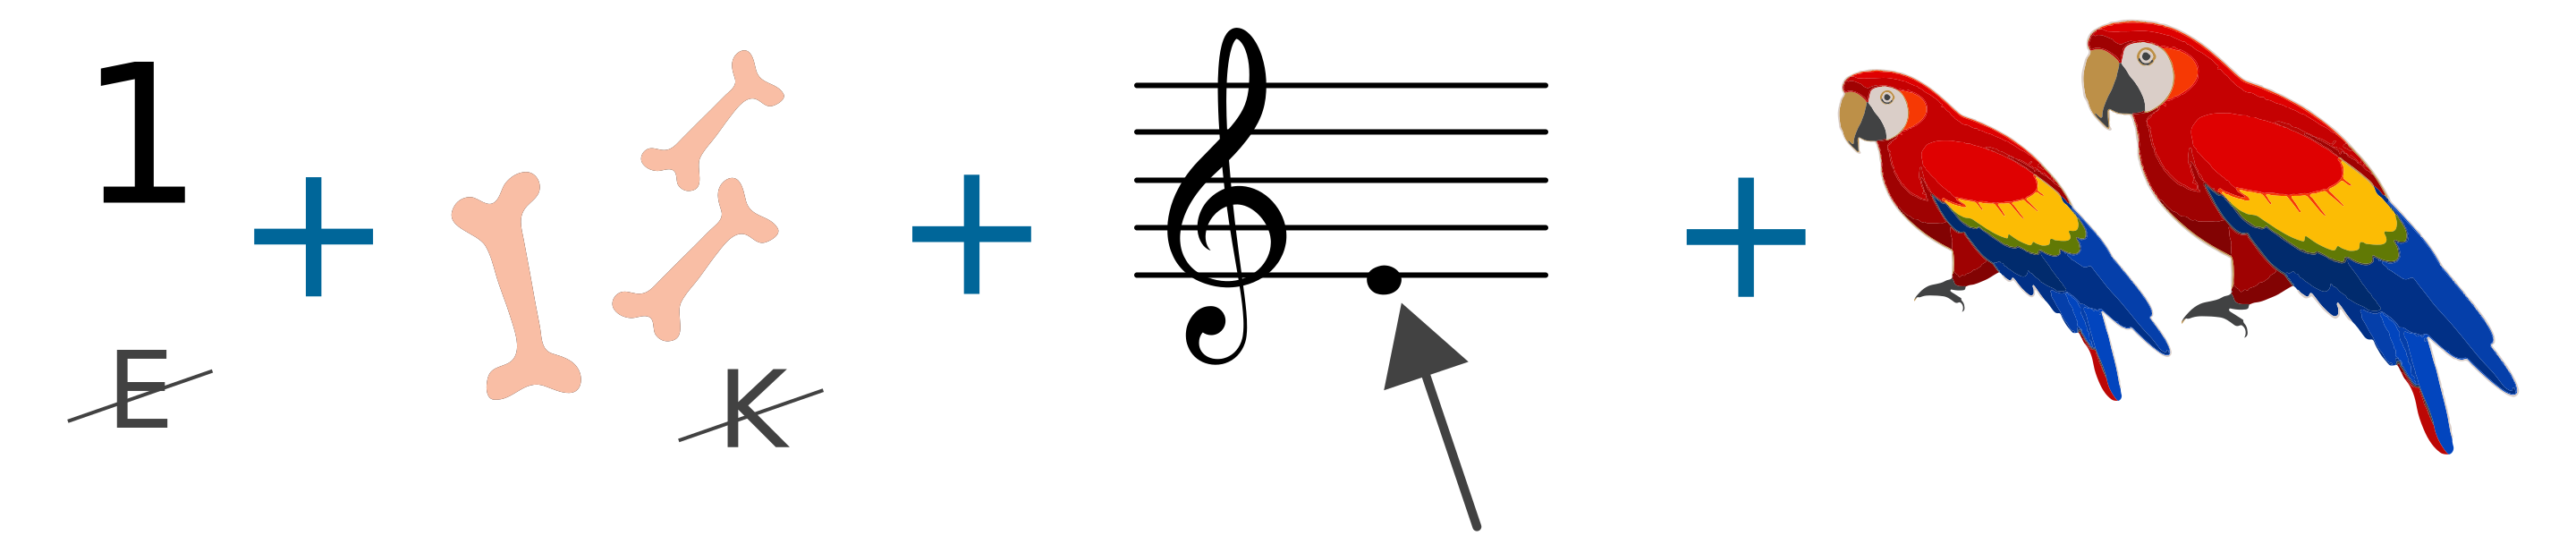
\includegraphics[width=8cm]{images/tyrek/rebus.png}
	\caption{Rebus. Źródło: Zespół autorski Politechniki Łódzkiej, licencja: CC BY 3.0}
\end{figure}

\subsubsection{Piętnastka - przesuwane puzzle}
Kolejnym przykładem może być też piętnastka, która w grze The Lore została zaimplementowana jako przesuwane puzzle rozmiarów 3 na 3. Temat szerzej poruszony będzie w dalszej części pracy, gdzie oprócz założeń związanych z rozwiązaniem zagadki, przedstawiona będzie logika idąca za zrealizowaniem tej zagadki w grze opartej na silniku Unity. 
\begin{figure}[h]
	\centering
	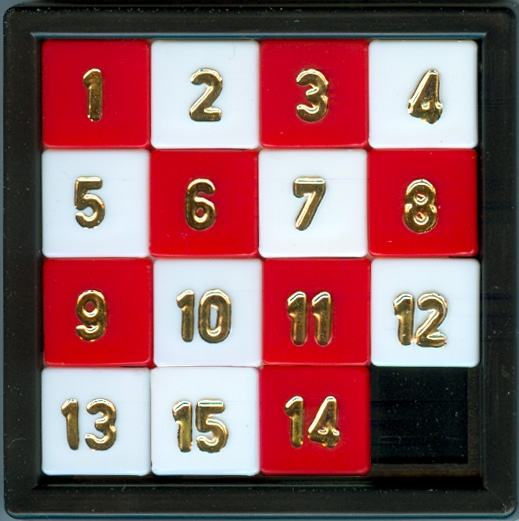
\includegraphics[width=5cm]{images/tyrek/przesuwane-puzzle.jpg}
	\caption{Piętnastka. Źródło: Wikipedia, Sliding Puzzle, Micha L. Rieser - Public Domain}
\end{figure}

\subsubsection{Puzzle}
Jedną z najpopularniejszych zagadek logicznych, z którą styczność miał zapewne każdy z nas, są puzzle. Jest to gra, w czasie której rozwiązujemy problem polegający na ułożeniu z dostępnych elementów logicznego obrazka, który zazwyczaj jest dołączony do gry - w postaci fotografii dołączonej do zestawu lub na pudełku.
 
Słowo puzzle pochodzi z XVI wieku, które oznaczało "stan zagubienia". Sama gra ma swoje początki w wieku XVIII, gdy John Spilsbury, grawer i kartograf umieścił mapę na drewnie, następnie przepiłował ją wokół konturów każdego kraju znajdującego się na mapie. To co powstało postanowił użyć do nauki geografii - ułożenie logicznej mapy uczyło jak wygląda mapa danego regionu. Taka pomoc dydaktyczna zdobyła szybko popularność, wszak była to nauka przez zabawę, używano ją dość często, nawet jeszcze w wieku XIX.  

Trudność puzzli zależy zazwyczaj od kształtu elementów i ich ilości. Jeżeli chodzi o kształt, puzzle często mają specyficzny kształt, przez co nie każdy element pasuje do innego, co pozwala nam odrzucić możliwość połączenia niektórych par. Ilość elementów zwiększa ilość możliwych oraz logicznych kombinacji danych puzzli, przez co zwiększa się czas realizacji zadania. Największa układanka została wykonana przez firmę Educa, posiadała ona aż 42 000 elementów i przedstawia dość bajeczny krajobraz, na którym znajdują się najpopularniejsze budynki z całego świata - Big Ben, Wieża Eiffela czy Krzywą Wieżę w Pizie. Ułożenie tej układanki możemy liczyć w setkach godzin. \cite{puzzle}

\begin{figure}[h]
	\centering
	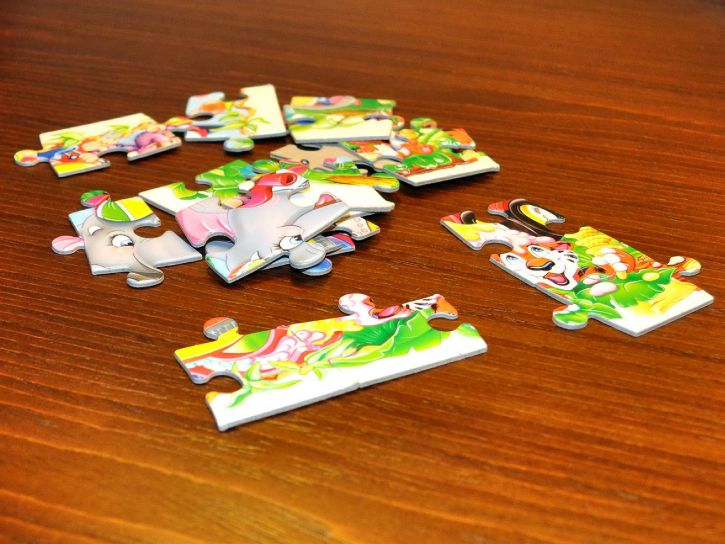
\includegraphics[width=5cm]{images/tyrek/puzzle.jpg}
	\caption{Źródło: Pixnio, Przykład puzzli - Public Domain}
\end{figure}

\subsection{Wdrożenie zagadek do gry opartej na silniku Unity}
Zanim przedstawione zostaną dwa sposoby wdrażania zagadek ze względu na sposób umieszczenia mini-gry w odpowiedniej hierarchii projektowej, warto poznać podstawowe pojęcia, które dotyczą projektu Unity.
\subsubsection{Scena w Unity}
W Unity możemy podzielić naszą grę na sceny. Scena to obiekt zawierający nasze menu, czy dane środowisko gry (na przykład poziom gry). Dobrą praktyką jest, aby każdy level gry był osobną sceną, co skróci czas jego ładowania. W scenie możemy umieścić swoje obiekty, skrypty czy grafiki. \cite{scena}
\subsubsection{Obiekt - GameObject}
\label{sec:gameobject}
Obiekt, zwany w Unity GameObject, to klasa podstawowa dla wszystkich podmiotów w scenach Unity. Do każdego obiektu możemy przypinać kolejne obiekty, tworząc hierarchiczność, która może się przydać w odpowiedniej realizacji projektu. \cite{gameobject}
\begin{figure}[h]
	\centering
	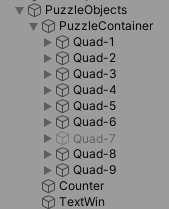
\includegraphics[width=4cm]{images/tyrek/hierarchia.png}
	\caption{Hierarchia obiektów. Przykład z projektu The Lore}
\end{figure}
\subsubsection{Komponent}
\label{sec:komponent}
Komponent jest klasą podstawową dla GameObject. Jest to klasa, przykładowo w języku C\#, która dołączana jest do obiektu Unity, celem wykonania na nim jakiś operacji. \cite{komponent}
\subsubsection{Sposoby dodawania mini-gier}
W toku pracy nad projektem The Lore rozpatrywano dwa sposoby dodawania mini-gier do gry:
\begin{itemize}
	\item{Każda minigra jest w osobnej scenie}
	\begin{itemize}
		\item W przypadku rozbudowanych poziomów nie powiela szerokiej listy obiektów sceny
		\item Pozwala na mniejsze pobieranie zasobów w danej jednostce czasu - połączenie działającego poziomu z algorytmiką mini-gry może bywać uciążliwe na słabszych komputerach.
	\end{itemize}
	\item{Każda minigra zawiera się w scenie poziomu gry}
		\begin{itemize}
		\item Unikamy dłuższego ładowania się poziomu gry po zakończeniu mini-gry
	\end{itemize}
\end{itemize}
Po wewnętrznej dyskusji wybrano opcję wydzielenia do osobnej sceny. W toku testowania tego rozwiązania uznano, iż nie jest ono bardzo uciążliwe pod kątem czasu ładowania poziomu, zaś pozwala na zachowanie porządku w projekcie. Jak się okazało już w przypadku tworzenia poziomu pierwszego gry, ta decyzja była właściwa. Z racji sporego rozbudowania tej sceny i dużej liczby obiektów na niej zawartych, dodanie mini-gier do tej sceny mogłoby spowodować chaos organizacyjny. Dodatkowo mogłoby wydłużyć czas ładowania poziomu i spowodować pobieranie większych zasobów w czasie gry.

\section{Przesuwane puzzle}
\subsection{Omówienie zagadnienia i ogólne założenia}
Przesuwane puzzle to układanka, złożona zazwyczaj z kwadratowej liczby elementów, najczęściej jest to szesnaście pól. Pola są jednakowych rozmiarów i oznaczone są liczbami od 1 do (n-1), gdzie n to liczba dostępnych pól w układance. Jedno pole jest puste, pozwala to na przeniesienie sąsiednich elementów puzzli względem siebie. Rozgrywka kończy się, gdy ułożymy puzzle w odpowiedniej kolejności, według rosnącego porządku liczb lub powstania odpowiedniego obrazka. Trudno określić kto odpowiada za stworzenie zagadki. Wiadomym jest, że w 1878 roku pochodzący ze Stanów Zjednoczonych Samuel Loyd wypromował układankę, jednak prawdopodobnie nie jest to jego pomysł. Dość popularną nazwą na rozgrywkę jest "piętnastka", określającą ilość dostępnych pól w najpopularniejszym ułożeniu - 4x4.  \cite{przesuwane_puzzle}

W grze The Lore gracze staną przez rozwiązaniem zagadki gdzie do dyspozycji mamy dziewięć pól. Podczas projektowania układanki w grze uznano, iż zagadka z piętnastoma elementami może być dość trudna, a korzyści płynące z rozwiązania jej będą nieadekwatne do poświęconego czasu, stąd ilość pól jest mniejsza niż w najpopularniejszej wersji rozgrywki.
\subsection{Algorytmika}
\subsubsection{Pojedynczy element puzzle - PuzzleBlock}

Każdy pojedynczy element puzzla jest zainicjalizowany jako obiekt, który określamy jako PuzzleBlock. Obiekt posiada koordynaty, które określają jego położenie w przestrzeni na układance.

\begin{figure}[h]
	\centering
	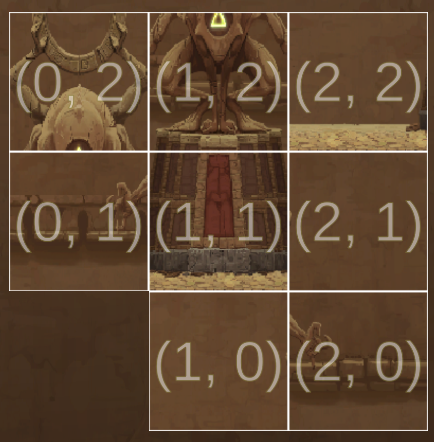
\includegraphics[width=6cm]{images/tyrek/coord_puzzle.png}
	\caption{Koordynaty każdego pola. Przykład z gry The Lore}
\end{figure}

Tak jak na załączonym przykładzie, wartość x rośnie w prawą stronę, zaś Y w górę, gdzie x dotyczy położenia w poziomie, a y w pionie. W założeniach przedstawiona została logika, która mówiła, iż element może zostać przemieszczony wtedy i tylko wtedy, gdy pole obok niego jest wolne, czyli nie posiada żadnego PuzzleBlock - elementu z liczbą lub obrazkiem. Dla lepszego efektu wizualnego, w grze The Lore element porusza się stopniowo, aby sprawiał wrażenie, iż porusza się realistycznie. Z racji, iż w Unity każda akcja wykonuje się podczas pokazywania kolejnej klatki, element porusza się w minimalnym stopniu przez sekundę. 

\subsubsection{Plansza - Puzzle. Losowanie kolejności puzzli}
	Plansza rozgrywki posiada 8 elementów PuzzleBlock oraz jedno puste pole.  Algorytm powinien wylosować dla 8 pól ich położenie na planszy - tak jak w wyżej przedstawionym przykładzie. W tym celu na początku losujemy dla każdego bloku wartość od 0 do 8. W C\# możemy to zrobić przy użyciu funkcji  \emph{System.Random().Next(a, b)}, który losuje wartości z zakresu \emph{<a, b)}. Przykładowo:
\begin{lstlisting}[
language={[Sharp]C},
rulecolor=\color{blue!80!black},
caption={Fragment klasy \texttt{Puzzle.cs}}
]
private int randomPosition()
{
    int pos = 0;
    do
    {
        pos = new System.Random().Next(0, 9);
    }
    while (isOnBoard[pos]);
    isOnBoard[pos] = true;
    return pos;
}
\end{lstlisting}

Gdzie isOnBoard[pos] jest tablicą, która weryfikuje, czy dane pole nie jest już zajęte. Jeśli jest, ponownie losujemy wartość dla PuzzleBlock. Oczywiście to nie koniec - z tej wartości musimy stworzyć położenie w postaci (x, y), gdzie x to położenie w poziomie, a y w pionie. W tym celu jedna z tych wartości będzie resztą dzielenia wylosowanej pozycji przez trzy (ilość pól w linii), a druga ilorazem całkowitym pozycji i liczby trzy. 
Kolejną ważną rzeczą będzie weryfikacja, czy obecne ułożenie puzzli jest wykonalne.

\subsubsection{Plansza - Puzzle. Weryfikacja kolejności puzzli}
Jak się okazuje niektóre ułożenia puzzli powodują, iż nie ma żadnego rozwiązania tego problemu. Z przypadkiem takiej sytuacji spotykaliśmy podczas pierwszych testów mini-gry puzzle. 
\begin{figure}[h]
	\centering
	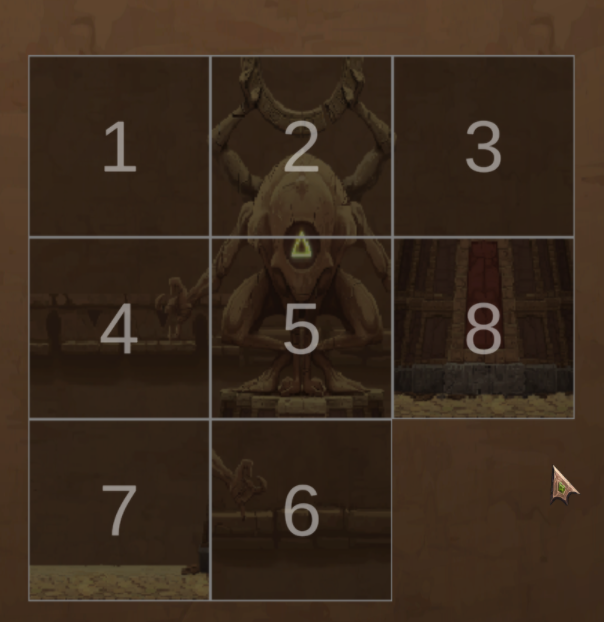
\includegraphics[width=5cm]{images/tyrek/puzzle_1.png}
	\caption{Puzzle bez rozwiązania. Przykład z gry The Lore}
\end{figure}

Jak się okazuje, występuje tutaj dość prosta zasada. Łamigłówka przesuwanych puzzli z 8 elementami jest rozwiązywalna wtedy i tylko wtedy, gdy liczba inwersji stanu początkowego jest parzysta. Czym jest zaś w tym przypadku liczba inwersji?

Inwersją nazwiemy parę liczb, której wartości są w odwrotnej kolejności, niż w zakładanym stanie końcowym. \cite{solvablePuzzle} Przyjmijmy taką sytuację:

\begin{center}
\begin{tabular}{ | m{5em} | m{1cm}| m{1cm} | } 
\hline
 1 & 2 & 3 \\ 
\hline
 6 & 4 & 5 \\
\hline  
 7 & 8 &     \\
\hline
\end{tabular}
\end{center}

W tym przypadku liczba inwersji wynosi dwa. Elementami zbioru inwersji są pary (6,4) oraz (6,5) - jak wiadomo, liczba 6 jest w kolejności po cyfrach 4 oraz 5. W tym przypadku rozwiążemy puzzle.

\begin{center}
\begin{tabular}{ | m{5em} | m{1cm}| m{1cm} | } 
\hline
 1 & 2 & 3 \\ 
\hline
 6 & 5 & 4 \\  
\hline
 7 & 8 &     \\
\hline
\end{tabular}
\end{center}

W tym przypadku liczba inwersji wynosi już trzy. Elementami zbioru są pary (6,5), (6,4) oraz (5,4). Takich puzzli nie da się rozwiązać. 
W projekcie platformowej gry w Unity zastosowaliśmy prostą weryfikacje tej sytuacji. 

\begin{lstlisting}[
language={[Sharp]C},
rulecolor=\color{blue!80!black},
caption={Fragment klasy \texttt{Puzzle.cs}}
]
int inversions = 0;
for (int i = 0; i < numbersOrdered.Length - 1; i++) {
    for (int j1 = i + 1; j1 < numbersOrdered.Length - 1; j1++) {
        if (numbersOrdered[j1] > numbersOrdered[i]) {
            inversions++;
        }
    }
}

\end{lstlisting}
Gdzie \textbf{inversions}, to liczba znalezionych inwersji, a \textbf{numberOrdered} to lista kolejności puzzli w stanie wejściowym. Jeżeli wartość \textbf{x} znajduje się w liście \textbf{numberOrdered} przed wartością \textbf{y} i jest od niej większa, to wtedy zwiększamy licznik inwersji o jeden.
Oczywiście pozostaje nam prosta weryfikacja, czy liczba inwersji jest nieparzysta - w takim wypadku puzzle będą nierozwiązywalne.
\begin{lstlisting}[
language={[Sharp]C},
rulecolor=\color{blue!80!black},
caption={Fragment klasy \texttt{Puzzle.cs}}
]
if (inversions % 2 == 1)
{
   pab.restartPuzzleButton();
}
\end{lstlisting}

Gdzie \textbf{pab} jest obiektem odwołującym się do akcji \textbf{PuzzleActionsButton}, zawierającym przycisk restartButton - ten sam, który dostępny jest w grze w celu zrestrartowania obecnego ułożenia puzzli.

Każdy obiekt (puzzle) ma przypisane do siebie dwie akcje: \textbf{OnBlockPressed} i \textbf{OnFinishedMoving}. Pierwsza akcja dotyczy tego, co ma się dziać w momencie wybrania przez gracza danego elementu. W tym przypadku dany element dodawany jest do kolejki, której zadaniem jest kontrola poruszania się puzzli. Pozwala to uniknąć sytuacji, gdy użytkownik zdołałby w bardzo szybkim czasie wybrać dwa elementy - wtedy moglibyśmy być świadkami nachodzących się puzzli lub nawet wejścia dwóch elementów na jedno miejsce. Gdy element będzie pierwszy w kolejce, rozpocznie się ruch naszego elementu - wtedy też przypisane będą mu nowe koordynaty. Wtedy przychodzi czas na drugą akcję, \textbf{OnFinishedMoving}. Początkowo funkcja zwiększa naszą ilość ruchów o jeden. Następnie sprawdza, czy obecne ułożenie puzzli odpowiada oczekiwanemu wynikowi końcowemu. Jeśli tak, jesteśmy informowani o ilości zdobytego doświadczenia. Ponownie widzimy animację przesuwającej się płytki, tym razem zamykającej się. Jeśli nie, algorytm sprawdza, czy istnieją elementy w kolejce, w tym przypadku powtarza się część procedury wykonywanej w \textbf{OnBlockPressed} - element porusza się na swoje miejsce, zmieniając koordynaty, następnie znów wykonując akcję \textbf{OnFinishedMoving}.

\subsection{Przedstawienie przykładu w grze The Lore}
W grze The Lore zagadka przesuwanych puzzli pełni rolę opcjonalnej rozgrywki, za której rozwiązanie gracz otrzymuje punkty doświadczenia. Mini-grę możemy rozpocząć znajdując się w pobliżu charakterystycznej płytki, wyróżniającej się podświetleniem.
\begin{figure}[h]
	\centering
	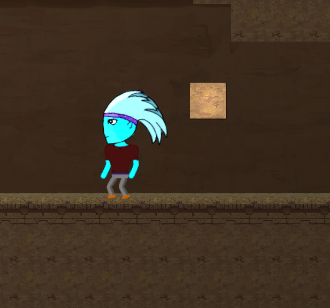
\includegraphics[width=6cm]{images/tyrek/the_lore_puzzle_lvl1.png}
	\caption{Miejsce rozpoczęcia puzzli. Przykład z projektu The Lore}
\end{figure}

W momencie naciśnięcia przycisku akcji kamera zbliża się do obiektu, czyli podświetlonej płytki. Następnie widzimy animację otwierającej się płytki sprawiającej wrażenie, iż ścianka jest przesuwana przez gracza.
\begin{figure}[h]
	\centering
	\includegraphics[width=7cm]{images/tyrek/otwieraniePuzzli.png}
	\caption{Animacja rozpoczęcia puzzli. Przykład z projektu The Lore}
\end{figure}

Po skończonej animacji rozpoczynamy mini-grę. Oprócz bloczków z kolejnością, na ekranie widzimy również dwa przyciski i cyfrę zero.
\begin{figure}[h]
	\centering
	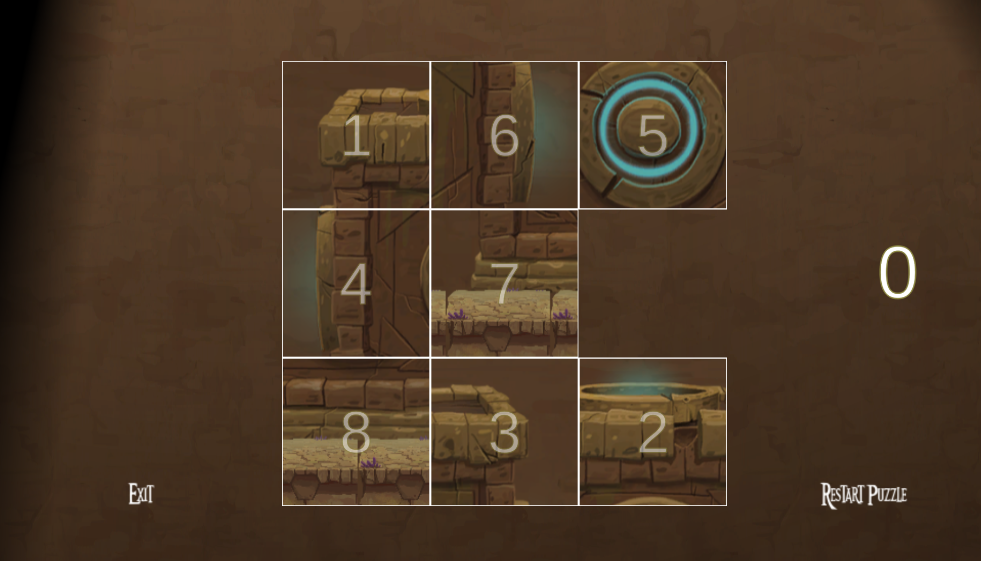
\includegraphics[width=7cm]{images/tyrek/puzzlebuttons.png}
	\caption{Cały interfejs mini-gry puzzle. Przykład z gry The Lore}
\end{figure}

Gdzie \textbf{Exit} kończy rozgrywkę, przenosząc nas z powrotem w miejsce, w którym rozpoczynaliśmy zagadkę, \textbf{Restart Puzzle} powoduje ponowne rozlosowanie puzzli, odwołując się do akcji w klasie \textbf{PuzzleActionsButtons}, czyli tej samej, która uruchamiana jest w przypadku, gdy puzzle nie mają rozwiązania. Dodatkowo po prawej stronie widnieje informacja ile ruchów do tej pory wykonaliśmy rozwiązując zagadkę. Jest to dość istotna informacja dla gracza, gdyż to od ilości ruchów zależy ile punktów doświadczenia zdobędzie za rozwiązanie tej zagadki. Zastosowany wzór dla gry The Lore wygląda następująco:

$$
y = \left\{ \begin{array}{ll}
5 & \textrm{gdy $x>=250$}\\
100 - (x / 25) * 10 & \textrm{gdy $x<250$}\\
\end{array} \right.
$$
Gdzie \textbf{x} jest liczbą wykonanych ruchów.
Po zakończeniu mini-gry jesteśmy informowani o ilości zdobytego doświadczenia. Ponownie widzimy animację przesuwającej się płytki, tym razem zamykającej się.
\begin{figure}[h]
	\centering
	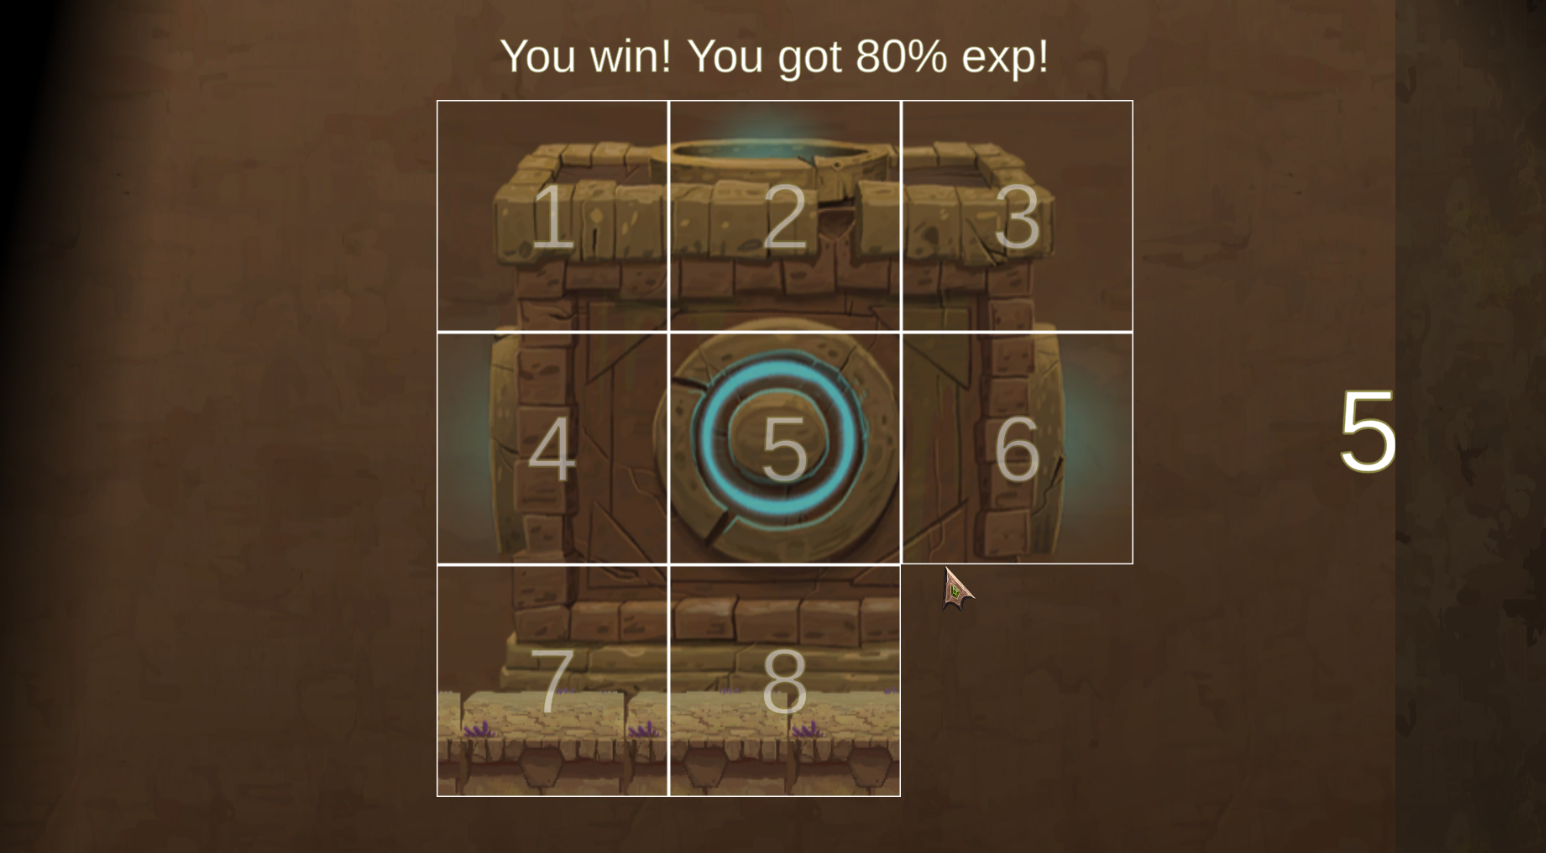
\includegraphics[width=7cm]{images/tyrek/puzzle_end.png}
	\caption{Wygrana rozgrywka puzzle. Przykład z gry The Lore}
\end{figure}

Każdą mini-grę puzzle można wykonać w grze tylko jeden raz. Ponowne próby są niemożliwe, a o tym, iż zagadka została zakończona, jesteśmy informowani przez fakt, iż płytka symbolizująca mini-grę nie jest podświetlona.

\begin{figure}[h]
	\centering
	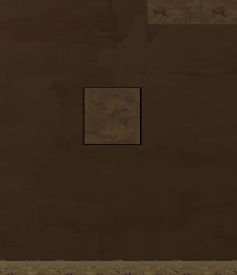
\includegraphics[width=5cm]{images/tyrek/puzzleWin.png}
	\caption{Wygaszona płytka. Przykład z gry The Lore}
\end{figure}


\subsection{Przedstawienie przykładu w innych grach}
\subsubsection{Nancy Drew: Hauting of Castle Malloy}
The Haunting of Castle Malloy to gra dwuwymiarowa przygodowa osadzona w Irlandii. Postać wybiera się do tego kraju, aby zostać drużbą na ślubie swojego przyjaciela. Jadąc autem na uroczystość zostaje zaatakowany przez upiorną postać, przez co wpada do rowu. Jak się później okazuje, zaginął Pan Młody. Główny bohater, Nancy Drew chce odkryć tajemnicę, przechodząc przez świat pełny zagadek. Właśnie podczas poszukiwania swojego Pana Młodego, gracz natyka się na przesuwane puzzle. 
\begin{figure}[h]
	\centering
	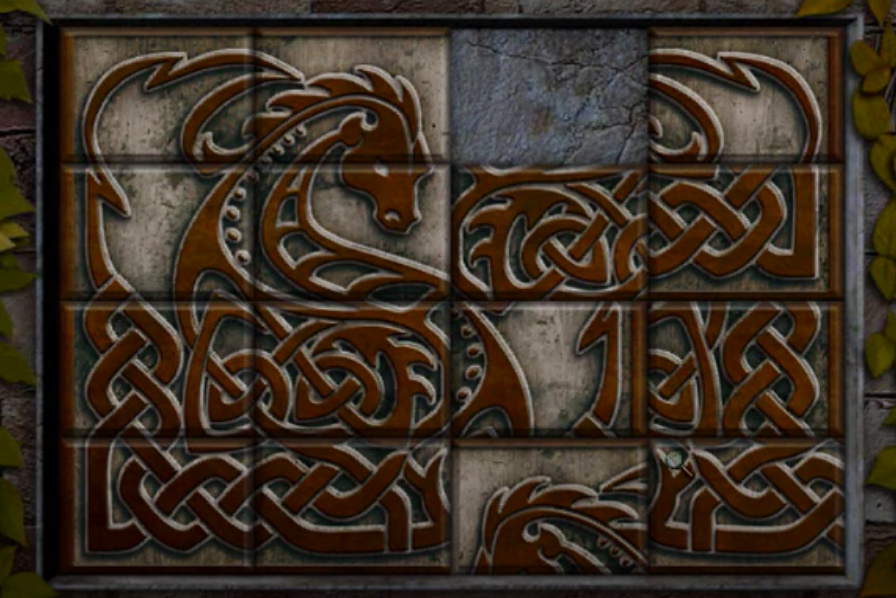
\includegraphics[width=6cm]{images/tyrek/nd.png}
	\caption{Przesuwane puzzle. Przykład z gry Nancy Drew: Hauting of Castle Malloy}
\end{figure}

W czasie przechodzenia kolejnych etapów, użytkownik ma możliwość przyglądania się obiektom, które mija. To właśnie w tym momencie może natrafić na omawianą rozgrywkę. Przed mini-grą gracz widzi jaki jest stan wyjściowy puzzli. Co warto podkreślić, w przeciwieństwie do gry The Lore, na poszczególnych elementach puzzli nie widzimy cyfr oznaczających poprawną kolejność puzzli. Aby zakończyć zagadkę należy również posiadać ostatni element, który po ułożeniu obrazka umieszczamy w brakującym miejscu. \cite{nd}


\subsubsection{Resident Evil 4}
Resident Evil 4 jest grą typu survival horror. Toczy się ona w fikcyjnym mieście Raccoon City, gdzie po sześciu latach kończy się śledztwo dotyczące nielegalnych badań i eksperymentów medycznych nad wirusem, prowadzone przez organizację Umbrella. Działania firmy spowodowały destabilizację tego miasta. Główny bohater, Leon S. Kennedy zostaje wyznaczony jako agent, który ma odnaleźć porwaną przez podejrzaną organizację, córkę prezydenta USA. Bohater przemierzając kolejne miasta odkrywa kolejne tajemnice związane z porwaniem. W toku gry zdarza się, iż gracz pokieruje Ashley Graham, czyli porwaną córką prezydenta USA. To właśnie w czasie kontrolowania tej postaci możemy natrafić na mini-grę związaną z przesuwanym puzzlami. Bohaterka może natrafić na totem, gdzie widać osiem elementów. Dialogi bohaterki podpowiadają graczowi, iż elementy mogą ułożyć się w logiczną całość. W przeciwieństwie do poprzedniego przykładu, nie mamy tutaj pokazanego efektu końcowego rozgrywki. Ostatni element, tak jak w Nancy Drew: Hauting of Castle Malloy musimy odnaleźć, aby zagadka została ukończona.

\begin{figure}[h]
	\centering
	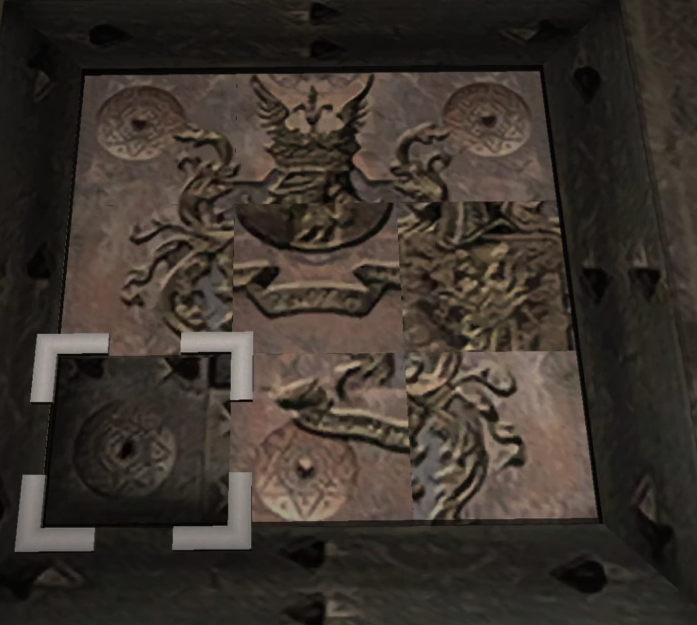
\includegraphics[width=5cm]{images/tyrek/re4.png}
	\caption{Przesuwane puzzle. Przykład z gry Resident Evil 4}
\end{figure}


\section{Zagadka z rurami}
\subsection{Omówienie zagadnienia}
Zagadka z rurami jest rozgrywką, której celem jest ułożenie ścieżki z dostępnych kształtów rur. Rodzaj rur jest tutaj ważny, ponieważ oprócz kształtów pionowych czy poziomych, dostępne są inne rodzaje - skośne, skrętne, półokrągłe.
Ścieżka powinna wyznaczać drogę wody począwszy od źródła, zazwyczaj zaznaczonego niebieskim kolorem, do końcowej rury. Rozgrywka kończy się, gdy woda dotrze do ostatniej rury w ścieżce, jeżeli będzie miejsce, w którym powinna kończyć się droga, gracz wygrywa. W innym wypadku ponosi porażkę.
Poziom naładowania wody pełni rolę wyznacznika czasu w którym użytkownik musi ułożyć odpowiednią ścieżkę. Zazwyczaj w tego typu rozgrywkach, woda przenosi się z rury źródłowej do kolejnej po pewnym czasie, aby dać graczowi pewien zapas czasowy na podjęcie odpowiednich decyzji. W niektórych grach gracz ma wybór rur, które dostępne są przez cała rozgrywkę - tak jest przykładowo w grze The Lore. Jednak są też cięższe przypadki, gdy mamy kolejkę kilku rur - wtedy musimy podejmować decyzję w oparciu o mniejszą pulę elementów.
\subsection{Algorytmika}
Mini-gra z rurami jest dość złożoną rozgrywką, dlatego zanim przedstawiony zostanie cały algorytm, warto na początku przytoczyć wszystkie obiekty, które pojawią się w czasie przedstawienia procedury.
\subsubsection{Pipe}
Jest to obiekt związany z rurą. To w tym miejscu określany jest typ rury, nadawana jest mu grafika oraz nazwa - ostatni element związany jest wyłącznie z częścią deweloperską, nie jest dostępne dla wszystkich użytkowników. W grze The Lore mamy dostępne kilka typów rur:
\begin{itemize}
  \item Rury pionowe - 9 elementów
  \item Rury poziome - 4 elementy
  \item Rury skrętne lewo-góra - 1 element
  \item Rury skrętne prawo-dół - 2 elementy
  \item Rury dół-lewo -  1 element
  \item Rury dół-prawo - 2 elementy
\end{itemize}
Jak wcześniej wspomniano, liczba elementów poszczególnych typów rur odgrywa ważną rolę. Nie jest możliwe ułożenie bez możliwości zejścia na dół (czyli między innymi bez rur skrętnych). 
\subsubsection{PipeSlot}
Jest miejscem, w którym może znaleźć się obiekt typu \textbf{Pipe}. Plansza, na której możemy kłaść elementy, jest rozmiarów 8x5, czyli tworzonych jest czterdzieści instancji obiektu \textbf{PipeSlot}. Jeżeli na danym miejscu znajduje się obiekt Pipe, wtedy możemy wykonywać na nim akcje - określa to zmienna \textbf{canDrag}. Do każdego obiektu przypisane są akcje \textbf{OnBeginDragEvent}, \textbf{OnEndDragEvent}, \textbf{OnDragEvent} oraz \textbf{OnDropEvent}. Związane są one ze systemem Drag\&Drop, którego działania zostanie przedstawione w dalszej części przedstawienia algorytmiki.
\subsubsection{Działanie algorytmu - UI}
Klasa \textbf{UI} odpowiada za interakcje z widocznym interfejsem i interakcje z obiektami. Na samym początku, do każdego elementu \textbf{PipeSlot} przypisywane są jego akcje. Gdy to już się stanie, czyszczona jest lista \textbf{pipes} w której trzymane będą wszystkie obiekty \textbf{Pipe}. Ma to na celu zabezpieczenie algorytmu przed wczytaniem elementów z poprzedniej instancji rozgrywki. Następnie wszystkie obiekty \textbf{PipeSlot} jako obiekt \textbf{Pipe} nadany mają \emph{null} – również z powodu zabezpieczenia przed niepożądanymi sytuacjami. Teraz czas na zainicjalizowanie dwóch najważniejszych \textbf{PipeSlot}, chodzi konkretnie o pierwszy i ostatni element. Dla tych miejsc przypisywana jest rura horyzontalna. Dodatkowo oba miejsca, pomimo iż znajduje się na nich rura, nie mogą być przeniesione – parametr \textbf{canDrag} ustawiony jest na \emph{false}. Oczywiście chodzi to o nieingerowanie w początek i koniec algorytmu. Gdy to już się stanie, algorytm dodaje rury wszystkich typów do odpowiedniej tablicy - \textbf{pipes}. Dopiero wtedy następuje losowanie im miejsc. W tym miejscu następuje przypisanie do elementu \textbf{PipeSlot} obiektów \textbf{Pipe}. Oczywiście, w momencie losowania miejsc, procedura weryfikuje, czy na danym miejscu znajduje się już jakaś rura, dzieje się to w dość trywialny sposób.

\begin{lstlisting}[
language={[Sharp]C},
rulecolor=\color{blue!80!black},
caption={Fragment klasy \texttt{UI.cs}}
]
if (pipeSlots[x].Pipe == null)
\end{lstlisting}
Jeżeli warunek nie jest spełniony, ponownie losowane miejsc miejsce dla obiekty \textbf{Pipe}. Gdy to już się stanie, rozgrywka rozpoczyna się. W tym momencie zaczyna mijać czas, którego limit wyznacza zmienna \textbf{targetTime} – ustawiona na pięć sekund. Czas ten dotyczy przepływu wody przez jedną rurę. Co warto podkreślić, co każdą pełną sekundę zmienia się grafika danego obiektu \textbf{Pipe} – nadając efekt płynięcia wody.

\begin{figure}[h]
	\centering
	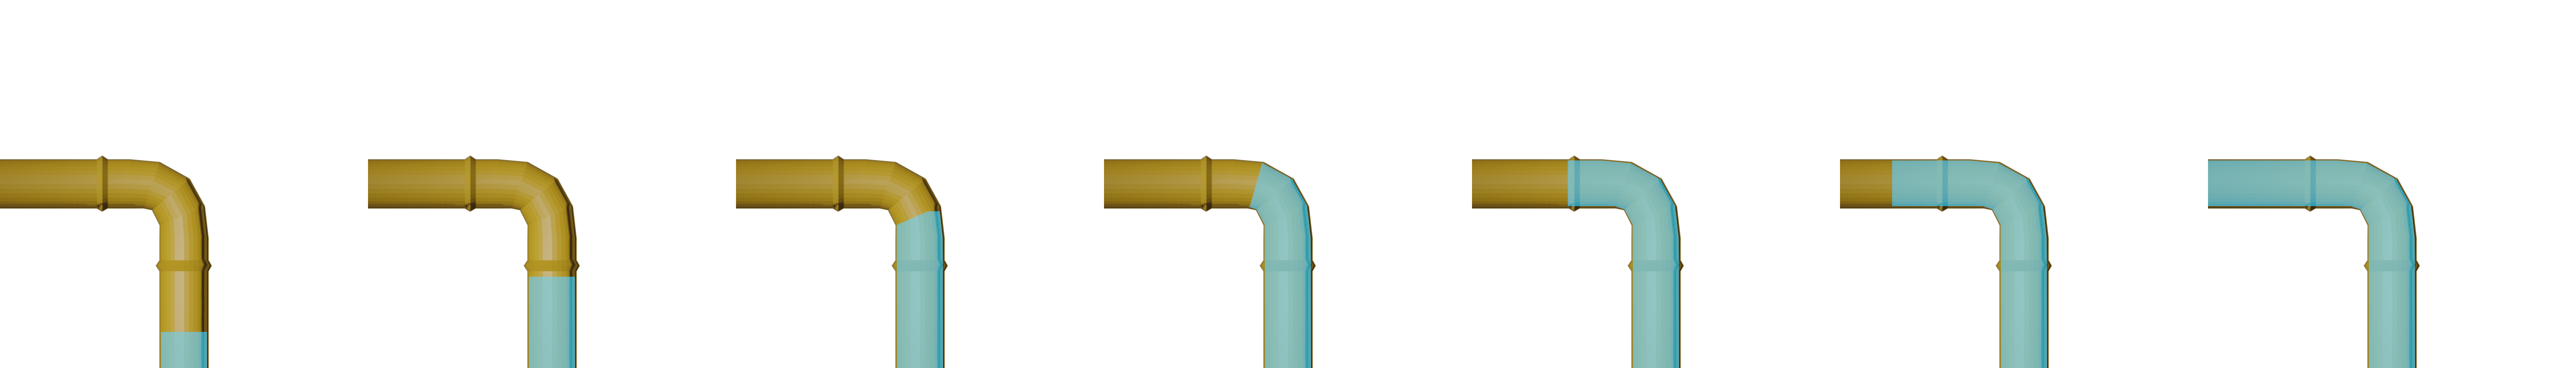
\includegraphics[width=10cm]{images/tyrek/rury-5.png}
	\caption{Grafiki rury skrętnej. Przykład z projektu The Lore}
\end{figure}
W danym momencie procedura weryfikuje też, czy istnieje połączenie. Dzieje się to poprzez warunki:
\begin{lstlisting}[
language={[Sharp]C},
rulecolor=\color{blue!80!black},
caption={Fragment klasy \texttt{UI.cs}}
]
if (recentPipe.right && (i + 1) % 8 != 7 && pipeSlots[i + 1].Pipe.left 
&& !cameFrom.Equals("right"))
\end{lstlisting}
Gdzie \textbf{recentPipe.right} to sprawdzanie czy obecna rura może skręcić w prawo, \textbf{((i + 1) \% 8 != 7)} jest weryfikacją, czy znajdujemy się przy najbardziej wysuniętym na prawo \textbf{PipeSlot}. Następnie weryfikujemy, czy sąsiedni slot może być skrętny w lewo. Niestety, warunki nie są zbyt proste. Podobnie sprawdzamy to dla wszystkich stron, z odpowiednimi wartościami dla danych przypadków. Jeżeli minie czas, a dany \textbf{PipeSlot} nie będzie miał odpowiedniego połączenia, jesteśmy informowani o porażce. Jeżeli zaś algorytm wykryje, iż takie połączenie istnieje, a naszym obecnym indeksem na planszy jest 39 (liczba pól – 1), to algorytm przenosi nas do poziomu gry, z którego zaczynaliśmy rozgrywkę.

\subsubsection{GameManager}
Ostatnim ważnym obiektem w kontekście tej mini-gry jest GameManager. Odpowiada on za wszystkie akcje przypisane do \textbf{PipeSlot}. \textbf{BeginDrag}, \textbf{EndDrag} oraz \textbf{Drag} odpowiadają za przenoszenie danej rury - w tym momencje pozycja obiektu jest ściśle związana z kursorem na ekranie. W momencie, gdy puścimy lewy przycisk myszy, wykonuje się akcja \textbf{Drop}. Tutaj weryfikujemy, czy \textbf{Pipe} został przeniesiony na \textbf{PipeSlot}, który nie posiada żadnej rury. Jeśli tak, do danego miejsca przypisana jest nowa rura. W innym wypadku rura wraca na swoje poprzednie miejsce. 
\subsection{Przedstawienie przykładu w grze The Lore}
Jest to kolejna mini-gra zawarta w grze The Lore, która jest elementem obowiązkowym do ukończenia poziomu "0", pełniącego rolę samouczka. Gracz zbliżając się do miejsca, w którym może rozpocząć rozgrywkę jest informowany poprzez komunikat o możliwości jej aktywacji.

\begin{figure}[h]
	\centering
	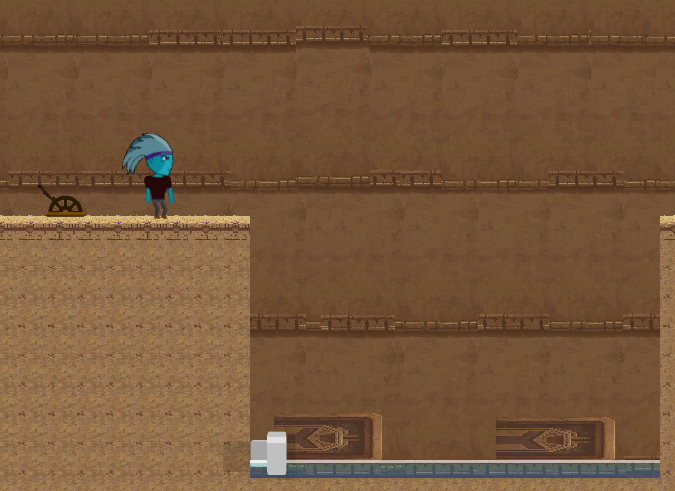
\includegraphics[width=7cm]{images/tyrek/ruryLvl0.png}
	\caption{Poziom 0 - Zagadka z rurami. Przykład z projektu The Lore}
\end{figure}

Jak widzimy po prawej stronie znajduje się doł, w którym widzimy dwa totemy oraz płytki strumień wody. W przypadku, gdyby gracz postanowił wskoczyć do dziury zostanie przeniesiony z powrotem w okolice przełącznika (widocznego na fotografii po lewej stronie). Gdy aktywujemy przełącznik przyciskiem akcji, kamera zmierza w dół, aby pokazać nam układ rur.

\begin{figure}[h]
	\centering
	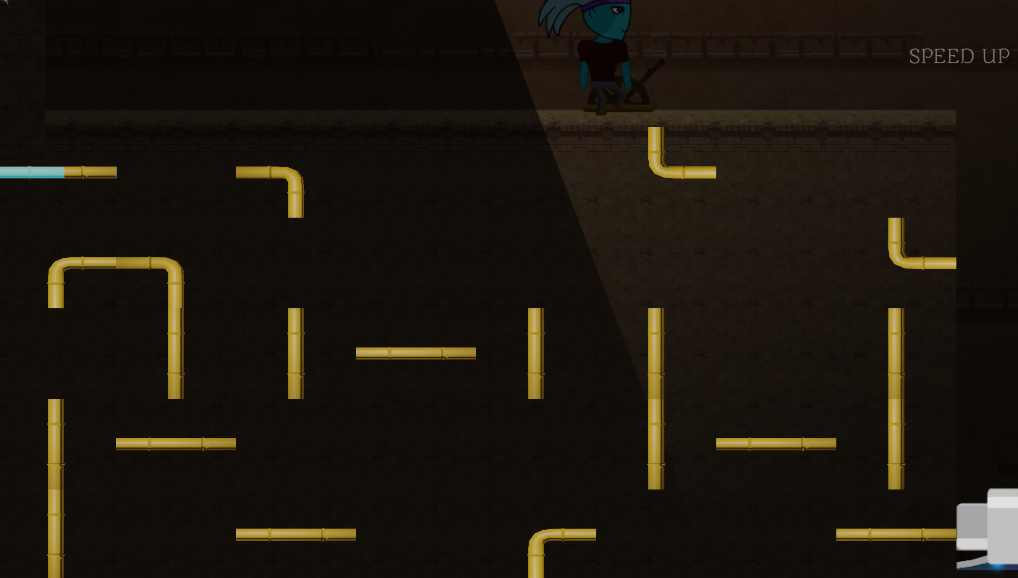
\includegraphics[width=12cm]{images/tyrek/pipes.png}
	\caption{Zagadka z rurami. Przykład z projektu The Lore}
\end{figure}

W lewym górnym rogu mamy źródło strumienia, zaś w prawym dolnym rogu zakończenie (szara rura). Użytkownik sterując myszką może przekładać rury o wybranym kształcie, tworzyć połączenia, celem stworzenia ścieżki, która jest konieczna do ukończenia mini-gry. Rozrywka zawsze generuje tą samą liczbę poszczególnych typów rur. Co warto podkreślić, liczba ta jest ważna - jeżeli mamy zbyt mało elementów danego typu, to po prostu ułożenie ścieżki może być niemożliwe. Zbyt duża liczba elementów zaś pozwoliłaby na trywialne rozwiązanie, na przykład w kształcie litery L. W grze The Lore jest możliwość szybkiego zakończenia rozgrywki poprzez wybranie opcji \textbf{Speed Up}. Powoduje ona szybkie przeniesienie strumienia wody do końcowej rury ułożonej przez nas ścieżki. Jeżeli odpowiednia droga została ułożona, mini-gra zostanie zakończona sukcesem, w przeciwnym przypadku porażkę. Z tej racji przycisk spełnia rolę nie tylko szybkiego pominięcia rozgrywki, gdy jesteśmy już pewni zwycięstwa i nie chcemy tracić czasu, ale też zrestartowania rur. 
\subsection{Przedstawienie przykładu w innych grach}
\subsubsection{Pipe Mania}
Gra logiczna stworzona przez The Assembly Line na platformy Amiga. Gra pojawiła się również na komputerach z systemem Windows. Rozgrywka polega na ułożeniu rurociągu z losowej puli rur. Kolejka rur, które otrzyma gracz wyświetla się po lewej stronie ekranu. Cała gra polega na ułożeniu ścieżki z dostępnych elementów, przy użyciu wszystkich rur. Liczba rur, które pozostały graczowi w kolejce wyświetlona jest w górnej części ekranu. Podobnie jak w grze The Lore, woda rozpoczyna swój bieg po pewnym czasie, gracz widzi ten czas w postaci paska po prawej stronie ekranu. \cite{pipemania}

\subsubsection{Soda Pipes}
Grą wzorowaną na poprzednim przykładzie jest Soda Pipes. Podobnie jak w poprzedniej grze, gracz musi ułożyć ścieżkę z rur, które losuje nam gra. W odrożnieniu do poprzedniczki, naszym celem jest zakończenie ścieżki w danym miejscu. Gra oprócz typowej rozgrywki oferuje również tryby gry, takie jak "puzzle mode" - pozwala on na układanie rur bez ograniczenia czasowego oraz trybu, w którym do pokonania jest 28 poziomów, które posiadają różne zadania. \cite{sp}
\section{Zagadka z otwieraniem zamku}
\subsection{Omówienie zagadnienia}
Jest to bardzo powszechna mini-gra, która dodawana jest do wielu gier, które posiadają funkcjonalność posiadania ekwipunku. Jej celem jest otworzenie skrzynii, które polega na wykonaniu różnych operacji. Zazwyczaj jest od odkrycie odpowiedniej sekwencji poruszania wytrychem, otworzyć zapadki poprzez poruszanie myszką, czy wciśnięcie odpowiedniego guzika, gdy postęp otwierania zamku jest na odpowiednim etapie. Otworzenie zamku pozwala otworzyć skrzynię, zawierającą elementy wyposażenia lub otworzyć drzwi, które zaprowadzą nas do ważnych dla gry pomieszczeń. Z racji na charakter rozgrywki element ten bywa raczej opcjonalną metodą przejścia gry. Z tego względu w niektórych grach, posiadających system umiejętności, otworzenie niektórych zamków jest niemożliwe lub bardzo trudne, jeżeli nie rozwiniemy odpowiednich umiejętności.
\subsection{Algorytmika}
Pierwszym i najważniejszym dla całej mini-gry elementem jest wylosowanie przez grę sekwencji ruchów, która potrzebna jest do ukończenia rozgrywki. Odbywa się to w skrypcie \textbf{PickLockGenerateSequence}. Podczas projektowania generatora napotkano się na problem związany z ciągłym losowaniem tych samych liczb. Powodem jest tutaj oczywiście synchronizacja, która przy ładowaniu scen potrafi sprawiać deweloperom problemy. Z tego powodu powstał ten skrypt, który wyróżnia się weryfikacją unikalności wylosowanej liczby.
Wszystko rozpoczyna się od losowania liczby z zakresu <1,100).
\begin{lstlisting}[
language={[Sharp]C},
rulecolor=\color{blue!80!black},
caption={Fragment skryptu \texttt{PickLockGenerateSequence.cs}}
]
    private int randomSide()
    {
        int random = 0;
        do
        {
            random = new System.Random().Next(1, 100);
        } while (wasRandomed[random - 1]);
        wasRandomed[random - 1] = true;
        return random % 2;
    }
\end{lstlisting}
Tablica \textbf{wasRandomed} to element, który inicjalizowany jest z samych wartości \textbf{false}. Ilość elementów jest równa \textbf{n}, czyli ilości możliwych wylosowanych liczb. Jeżeli liczba zostanie wylosowana ponownie, skrypt próbuje wylosować kolejną. Tak jak wspominano gracz ma dwie możliwości ruchów, dlatego aby wszystko działało poprawnie funkcja zwraca \textbf{mod 2} z wylosowanego elementu. Wynikiem funkcji jest więc 0, co oznacza ruch w lewo oraz 1, co oznacza ruch w prawo. Losowanych jest pięć elementów, co tworzy nam tablicę ruchów które musi wykonać gracz.
\begin{lstlisting}[
language={[Sharp]C},
rulecolor=\color{blue!80!black},
caption={Fragment skryptu \texttt{PickLockGenerateSequence.cs}}
]
for (int i = 0; i < numberOfMoves; i++)
{
   moves[i] = randomSide();
 }
\end{lstlisting}
Po wszystkim aktywowany jest \hyperref[sec:komponent]{\emph{komponent}} \textbf{Picklock}. Komponent ten odpowiada za wykrywanie jakich wyborów dokonał gracz. Jeżeli gracz wykonał dobry ruch, zostanie poinformowany o tym poprzez komunikat oraz zwiększy się licznik kontrolny \textbf{step} ilości dobrych ruchów. W przeciwnym razie licznik się wyzeruje. Dla efektu wizualnego, gracz widzi w którą stronę poruszył się jego wytrych - pozwala to łatwiej zapamiętać wybór. Odbywa się to poprzez zmianę pozycji elementu transform.

\begin{lstlisting}[
language={[Sharp]C},
rulecolor=\color{blue!80!black},
caption={Fragment skryptu \texttt{Picklock.cs}}
]
picklockTransform.position += new Vector3(10 * direction, 0, 0) * 0.1f;
\end{lstlisting}

Gdzie picklockTransform to \hyperref[sec:komponent]{\emph{komponent}} typu transform, zawierający tablicę pozycji, rotacji oraz skalowania (odpowiednio parametry position, rotation i scale) \hyperref[sec:gameobject]{\emph{obiektu}}. W tym przypadku interesuje nas tylko \textbf{position}. 
\subsection{Przedstawienie przykładu w grze The Lore}
W grze The Lore otwieranie zamków dotyczy skrzyń, które położone są w różnych częściach mapy. Podczas poziomu samouczka jesteśmy informowani o możliwości rozpoczęcia mini-gry. Rozpoczęcie mini-gry wymaga posiadania wytrychów, które wyróżnione są na mapie białym podświetleniem.

\begin{figure}[h]
	\centering
	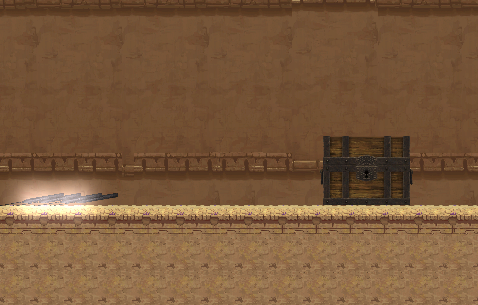
\includegraphics[width=10cm]{images/tyrek/skrzynia.png}
	\caption{Wytrychy i skrzynia. Przykład z projektu The Lore}
\end{figure}

Jeżeli chcemy otworzyć skrzynie nieposiadając w ekwipunku żadnego wytrychu, jesteśmy informowani o tym fakcie poprzez komunikat na ekranie. Gdy wciśniemy odpowiedni przycisk akcji, kamera zbliża się do skrzyni, po pewnym czasie rozpoczyna się mini-gra.
Na wstępie jesteśmy informowani poprzez komunikat o sterowaniu w rozgrywce. Klawisze "Left/RightButton" są zależne od ustawień sterowania i dotyczą przycisków poruszania się graczem w lewo i prawo. Jeżeli naciśniemy któryś z tych przycisków, wytrych przesunie się zgodnie z naszym poleceniem. Po każdym ruchu jesteśmy informowani, czy był on odpowiedni.

\begin{figure}[h]
	\centering
	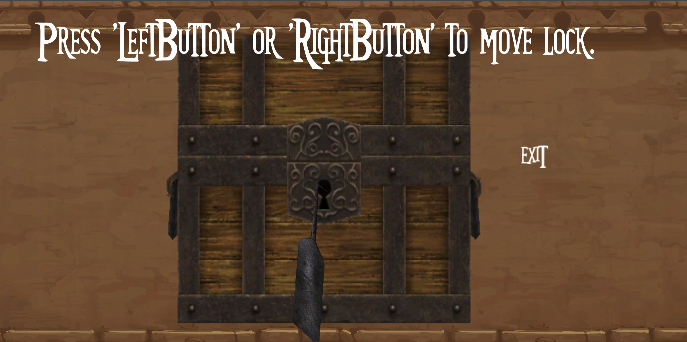
\includegraphics[width=12cm]{images/tyrek/minigraskrzynia.png}
	\caption{Mini-gra otwieranie skrzyń. Przykład z projektu The Lore}
\end{figure}

Zadaniem gracza jest zgadnąć losowy ciąg elementów lewo/prawo o długości 5. Każdy zły ruch powoduje konieczność powtórzenia sekwencji. Nagrodą za rozwiązanie problemu są eliksiry przywracające punkty życia, które przydają się w czasie rozgrywki. Z racji, iż jest to rozgrywka nieobowiązkowa, gracz w każdej chwili może ją opuścić wybierając opcję \textbf{Exit}.
\subsection{Przedstawienie przykładu w innych grach}
\subsubsection{Mafia 2}
Gra Mafia II osadzona jest w amerykańskim mieście rządzonym przez mafie. Głównym bohaterem jest Vito Scaletta, syn włoskich imigrantów. Los sprawia, iż bohater zmuszony jest do szybkiego zarobku, przez co wplata się w mafijne porachunki. Realizując zadania dla swoich pracodawców, nieraz włamywał się do różnych pomieszczeń. Gracz może również w czasie gry włamywać się do zamkniętych pokoi lub budynków celem szybszego przejścia poziomu, obejścia wrogów czy zdobycia pieniędzy. Dodatkowo mini-gra pozwala na odblokowanie zamkniętych pojazdów. W mini-grze gracz używa myszki. Widoczny jest zamek z trzema zapadkami, po prawej stronie widzimy wytrych przy pierwszej zapadce. Użytkownik sterując myszką wertykalnie musi ustawić zapadkę w takiej pozycji, aż będzie ona podświetlona na kolor zielony. Jeżeli gracz zrobi to w złym momencie, zostanie cofnięty do poprzedniej zapadki. \cite{Mafia2}
\begin{figure}[h]
	\centering
	\includegraphics[width=5cm]{images/tyrek/Mafia2.png}
	\caption{Otwieranie zamków. Przykład z gry Mafia 2}
\end{figure}
\subsubsection{Assassin's Creed Unity}
W grze Assassni's Creed Unity wcielamy się w Arno Doriana, członka tajnego bractwa Assasynów, którzy toczą odwieczną walkę z organizacją zwaną Templariusze. Gra osadzona jest w czasach rewolucji francuskiej w Paryżu. Bohater będąc w centrum najważniejszych wydarzeń osiemnastowiecznego Paryża nieraz potrzebuje włamać się do jakiegoś budynku, aby wykonać misję. W grze otwieranie zamków dotyczy pomieszczeń, które dają podobnie jak w poprzednie grze, możliwość obejścia wrogów, czy też zdobycie ekwipunku oraz włamywania się do skrzyń - podobnie jak w grze The Lore. Rozpoczynając mini-grę widzimy ilość zapadek, błękitny pasek poruszający się wertykalnie oraz błękitny prostokąt. Zadaniem gracza jest wcisnąć przycisk akcji w momencie, gdy poruszający się znacznik znajdzie się w błękitnym polu. W przypadku, gdy gracz zrobi to w złym momencie, traci z ekwipunku wytrych. Warto też podkreślić, iż w grze istnieje system umiejętności, gdzie dwie umiejętności dotyczą poziomu otwierania zamków. Podczas gry spotkamy trzy poziomy trudności, które charakteryzują się większą ilością zapadek czy też szybszym poruszaniem się błękitnego paska. \cite{acu}
\begin{figure}[h]
	\centering
	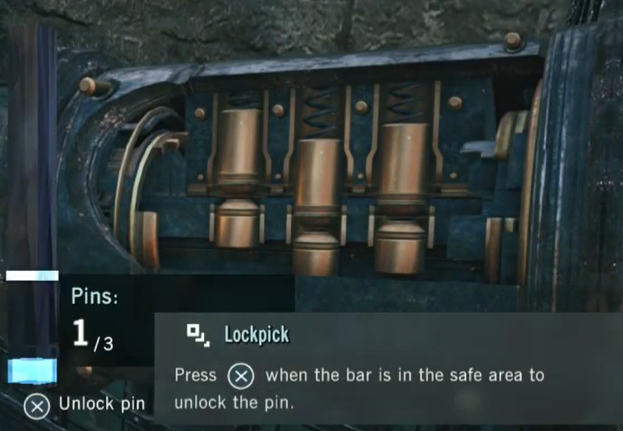
\includegraphics[width=6cm]{images/tyrek/acu.png}
	\caption{Otwieranie zamków. Przykład z gry Assassin Creed Unity}
\end{figure}
\subsubsection{Gothic 2}
Gothic 2 to gra osadzona w krainie Myrtana, w której toczy się walka pomiędzy siłami dobra i zła. Wcielamy się w byłego więźnia kolonii więziennej, który w wyniku pokonania Śniącego, tajemniczego potwora, niszczy magiczną barierę, która odcinała kolonię karną od reszty świata. Po upadku bariery bohater zostaje wybudzony przez nekromantę Xardasa, który informuje go o nowych zagrożeniach, które grożą krainie Myrtana. Gracz sterując bohaterem może dopuszczać się przestępstw, które pozwalają mu na zdobycie odpowiedniego ekwipunku czy złota. Może się to odbywać między innymi poprzez plądrowanie skrzyń w chatach mieszkańców miasta Khorinis, czy też napotkanych, opuszczonych budynkach. 
Logika otwierania zamków, zarówno drzwi jak i skrzyń, jest dość podobna do zastosowanego systemu w grze The Lore. Gracz aby otworzyć daną skrzynie musi posiadać wytrychy, które może zakupić od kupców w mieście. Otwieranie skrzyń polega na odgadnięciu odpowiedniej sekwencji lewo – prawo, w przypadku pomyłki gracz może utracić wytrych. Co ciekawe, gra nie losuje kolejności sekwencji. Jest ona stała dla danej skrzyni w świecie gry, co może stanowić swego rodzaju ułatwienie - odpowiednie sekwencje można po prostu odnaleźć w internecie.


\section{Labirynt}
W pierwotnej definicji, labirynt oznacza budowlę, która charakteryzuje się układem dużej ilości pomieszczeń, które połączone są krętymi ciągami korytarzy. Oczywiście miało to na celu utrudnić dostęp do pewnego pomieszczenia osobom niepowołanym. Z podobnych powodów w niektórych grach mamy do czynienia z labiryntem, zmuszając w ten sposób gracza do szukania wskazówek, czy też zapamiętywaniu ścieżek, celem wyjścia z labiryntu. 
\subsection{Omówienie zagadnienia}
\subsection{Algorytmika}
\subsubsection{Założenia: algorytm z nawrotami}
Do stworzenia labiryntu możemy użyć algorytmu z nawrotami. Początkowo powinniśmy stworzyć graf, gdzie każdy węzeł ma co najmniej jedno połączenie, to będzie nasz labirynt. Pomiędzy węzłami, które nie są połączone będzie znajdować się ściana, której użytkownik nie może przejść. Aby wygenerować taki graf, początkowo  generujemy graf bez ścieżek - możemy wyobrazić sobie, iż jest to po prostu prostokąt, podzielony na kilka kwadratów stworzonych przez ściany. Algorytm rozpoczyna się w pierwszym węźle, dodając go do stosu. Następnie wybiera pierwszego nieodwiedzonego sąsiada, tworząc w ten sposób pierwsze połączenie węzłów - z punktu widzenia gracza, usuwając pomiędzy nimi ścianę. Proces powtarzany jest aż do momentu, gdy trafimy do węzła, które nie ma żadnego nieodwiedzonego sąsiada. Gdy już dotrze do takiego miejsca, cofa się, jednocześnie usuwając elementy ze stosu, aż do momentu, gdy trafi na węzeł, który posiada nieodwiedzonego sąsiada. Algorytm skończy się, gdy w naszym stosie nie będzie elementów. \cite{maze}
\subsubsection{Implementacja: algorytm z nawrotami}
Przejdźmy teraz do zaprojektowania takiej sytuacji. Na sam początek zdefiniujmy stany, które może posiadać każdy węzeł w naszym grafie (labiryncie). Jak wiemy, może mieć ściany ściany z czterech stron. 
\begin{lstlisting}[
language={[Sharp]C},
rulecolor=\color{blue!80!black},
caption={Stany danego węzła - skrypt C\#}
]
public enum NodeState
{
    LEFT = 1,
    RIGHT = 2,
    UP = 4,
    DOWN = 8,
    VISITED = 128
}
\end{lstlisting}
W ten sposób możemy łatwo określić wszystkie ściany, które otaczają nasz węzeł. Przykładowo, gdybyśmy chcieli przedstawić, iż nasz węzeł otacza ściana lewa i górna, stworzylibyśmy stan \textbf{NodeState nodeState = NodeState.LEFT | NodeState.UP}. Jak wspomnieliśmy, chcemy, aby na początku wszystkie ściany tworzyły swego rodzaju siatkę, która odgradza każdy węzeł od innych. Generowanie jest w tym przypadku bardzo proste, wystarczy w odpowiedniej pętli wykonać odpowiednią liczbę iteracji \textbf{nodeWall[i] = NodeState.LEFT | NodeState.RIGHT | NodeState.UP | NodeState.DOWN}. Możemy również uznawać wartości za liczby binarne, \textbf{LEFT} jako 0001, \textbf{UP} 0010 i tak dalej. Oznaczmy też stan odwiedzonego pola jako 128 - reprezentacja bitowa 1000 0000. W przypadku, gdy chcemy dodać do naszego obiektu nowy stan, wystarczy wykonać operację dodania alternatywy do obecnego stanu. \textbf{node[x,y] |= WallState.VISITED} Oczywiście w ramach większego porządku w kodzie warto określić \textbf{nodeWall} jako tablicę dwuwymiarową, wyznaczając położenie w osi poziomej i pionowej. Pomoże nam to rozpoznać w jakim miejscu na labiryncie znajduje się dany węzeł. Jest to szczególnie przydatne, ponieważ będziemy tworzyć strukturę pod pozycję każdego obiektu. Pozycje, tak jak wyżej wspomniano, przedstawiamy w geometrii dwuosiowej, co oczywiście pomoże nam śledzić gdzie znajduje się dany obiekt. 
\begin{lstlisting}[
language={[Sharp]C},
rulecolor=\color{blue!80!black},
caption={Pozycja obiektu - skrypt C\#}
]
public enum NodePosition
{
	public int x;
	public int y;
}
\end{lstlisting}
Warto też stworzyć strukturę do przechowywania informacji o sąsiadach naszego węzła. Wystarczą wyżej przedstawione parametry \textbf{NodeState} i \textbf{NodePosition}. Dodatkowo w ramach kontroli powinniśmy stworzyć listę takich obiektów, które nie zostały jeszcze odwiedzone przez algorytm. Mając już takie struktury, kolejnym krokiem byłoby stworzenie metody, która zwraca nam stan danego sąsiada. Tak jak wspominano na początku, sąsiad będzie wybierany losowo, dlatego warto już na wstępie stworzyć obiekt \textbf{System.Random()}. Dzięki stworzonej wcześniej metodzie pobierania sąsiadów możemy go wybrać na przykład ze względu na kolejność na danej liście. Tworzymy też najważniejszy dla algorytmu z nawrotami stos. Każdy odwiedzony węzeł powinien być oznaczony wartością \textbf{NodeState.VISITED} i dodany do tego stosu. Wystarczy, aby były to obiekty \textbf{NodePosition}, jednak nic nie zaszkodzi, aby były to całe obiekty \textbf{WallState}. Teraz dzięki pętli while, powinniśmy sprawdzać kolejne węzły, dopóki nasz stos nie będzie pusty. Jeżeli ostatnio dodany do stosu obiekt posiada co najmniej jednego sąsiada, to pobieramy ich listę, przy użyciu funkcji losującej i wybieramy dany element z posiadanej listy. Dodajemy do stosu wylosowany obiekt.
Następnie powinniśmy usunąć każdą odwiedzą ścianę. 

\begin{lstlisting}[
language={[Sharp]C},
rulecolor=\color{blue!80!black},
caption={Usunięcie ściany - skrypt C\#}
]
node[x ,y] &= ~neighbour.SharedWall;
\end{lstlisting}

Gdzie \textbf{SharedWall} mówi nam o tym, czy pomiędzy dwoma obiektami znajduje się ściana. Oczywiście, informacja o ścianie powinna zostać zaktualizowana również u sąsiada. W tej sytuacji są dwa wyjścia. Pierwszy z nich, z lekka naiwny i niezbyt przyjazny dla oka dewelopera to stworzenie czterech warunków, które definiują dla danego przypadku jak pobrać pozycję przeciwną, dla sąsiada po lewej stronie - prawo, dla sąsiada na dole - góra i tak dalej. W ten sposób możemy zdobyć węzeł i zmienić jego stan, a następnie dodać nowy element do stosu. Drugim, rozsądniejszym pomysłem jest zadeklarowanie metody, która mogłaby od razu zwrócić nam \textbf{WallState} naszego sąsiada, który od razu mógłby być szybko poprawiony. Z pomocą przychodzi tutaj prosta instrukcja switch(), która pozwala nam na zarządzanie czterema przypadkami, z którymi będziemy mieli do czynienia.

\begin{lstlisting}[
language={[Sharp]C},
rulecolor=\color{blue!80!black},
caption={Zwracanie stanu sąsiada - skrypt C\#}
]
switch(nodeState)
{
	case NodeState.RIGHT =  return  NodeState.LEFT;
	case NodeState.LEFT = return  NodeState.RIGHT;
	case NodeState.UP =  return NodeState.DOWN;
	case NodeState.DOWN = return NodeState.UP;
}
\end{lstlisting}

Algorytm gotowy. W tym momencie mamy stworzony generator labiryntu, który powinien zostać jeszcze stworzyć algorytm odpowiedzialny za wygenerowanie w naszej grze labiryntu. Dzięki otrzymanym informacją nie sprawia to większych problemów. Mając informację o wszystkich węzłach, możemy stworzyć pętle, która tworzy obiekty ścian ze względu na ściany istniejące dla danego węzła. Z pomocą przychodzi tu obiekt \textbf{Instantiate}. Służy on do klonowania przekazanego obiektu (dla nas ściany). Dodatkowa metoda ta pozwala nam na określenie dokładnej pozycji oraz rotacji naszego elementu, co pozwoli nam na ułożenie ściany w wyznaczonym miejscu i pozwoli na obrócenie obiektu - ze względu czy jest ścianą pionową czy poziomą. Dokładny obiekt który jest nam potrzebny to \textbf{Instantiate(Object original, Vector3 position, Quaternion rotation)}. \cite{Instantiate}
Teraz używając czterech warunków, dla każdej strony, weryfikujemy, czy nasz węzeł sąsiaduje z daną ścianą. Dla każdej ściany (jeśli istnieje) tworzymy jej obiekt. Następnie powinniśmy określić pozycję - tutaj przychodzi z pomocą obiekt Vector3. Jest to trójelementowa struktura, która przydaje się w określaniu między innymi pozycji w trzech osiach - \textbf{Vector3(x, y, z)}. \cite{Vector3}. Pozycja jest tutaj zależna od naszych wymagań - powinniśmy dopasować ją do wielkości naszego obiektu. Z pomocą przychodzi Unity, które w sekcji Inspector pozwala łatwo zarządzać wielkością naszego obiektu. Rotacja potrzebuje zaś już czteroelementowego obiektu - Quaternion. Ze względu na posiadany przez nas obiekt ściany musimy sami określić która oś powinna zostać zmieniona. W ten sposób powinniśmy mieć już widoczny wygenerowany labirynt.


\subsection{Przedstawienie przykładu w innych grach}
\subsubsection{Wriggler}
Wriggler jest grą wydaną w 1985 roku. W grze sterujemy robakiem, którego zadaniem jest uciec z labiryntu składającego się z 256 poziomów, w ramach wyścigu w którym bierze udział. Każdy poziom (labirynt) jest stały - nie są one generowane w czasie gry. Gra została stworzona przez braci Kempthorne oraz David'a Vivian'a. \cite{Wriggler}

\begin{figure}
	\centering
	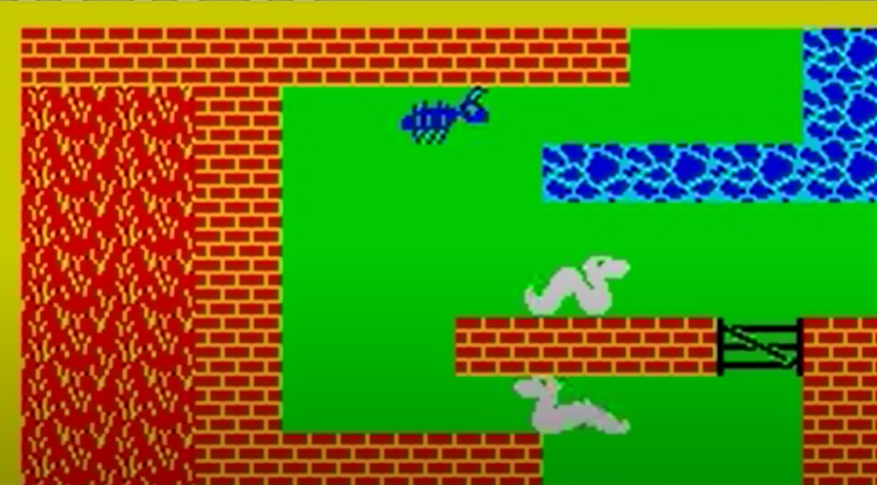
\includegraphics[width=8cm]{images/tyrek/wriggler.png}
	\caption{Labirynt. Przykład z gry Wriggler}
\end{figure}

\subsubsection{Dandy}
Kolejną grą opartą na labiryntach jest Dandy. Gra powstała w 1983 roku na platformy Atari, przez Johna Howarda Palevicha, w ramach pracy licencjackiej na MIT. Gracz steruje postacią, poruszając się po lochach z wieloma poziomami, które połączone są ze sobą schodami. Niektóre fragmenty labiryntu zamknięte są przez drzwi, do których otwarcia potrzebne są klucze, rozsiane po planszy. Oprócz pokonywania kolejnych poziomów, gracz może pokonywać wrogów przy użyciu łuku. \cite{Dandy}
\section{Podsumowanie}
Jak widać, projektowanie zagadek logicznych jako mini-gry może nie być aż tak trudne. Dużo zależy od podejścia autora i kreatywności w przewidywaniu szczególnych sytuacji - czego przykładem jest kwestia nierozwiązywalnych przesuwanych puzzli. Pomocne jest tu też narzędzie Unity i zawarte w nim funkcjonalności. Dzięki odpowiednim dopasowaniom komponentów do obiektów, możemy łatwo podczas podglądu gry, testować produkt pod kątem potencjalnych błędów. Na pewno wielkim plusem jest tu też szeroka dokumetnacja Unity, która pozwala nam łatwo znaleźć funkcje, czy obiekty, które mogą się przydać w toku tworzenia własnej rozgrywki.
\chapter{Fizyka postaci}
\section{Tworzenie postaci}
\subsection{Omówienie zagadnienia procesu tworzenia postaci}
\subsection{Proces graficzny tworzenia postaci}
\subsection{Wdrożenie postaci do projektu w Unity}
\subsection{Sposoby animowania postaci}

\section{Poruszanie się}
\subsection{Omówienie zagadnienia}
\subsection{Fizyka w grach 2D, a w prawdziwym świecie}
\subsection{Poruszanie się oraz kolizje postaci}
\subsection{Skakanie} 
\subsection{Otoczenie wpływające na fizykę postaci}
\subsection{Umiejętności związane z poruszaniem się}

\begin{thebibliography}{10}
\bibitem{projekt}
Robert K. Wysocki, Rudd McGary: Efektywne zarządzanie projektami. Wydanie III, ISBN: 83-7361-861-9, dostęp w internecie 26.01.2021r.
http://pdf.onepress.pl/efzapr/efzapr-1.pdf

\bibitem{IO- Helion}
Bernd Bruegge, Allen H. Dutoit: Inżynieria oprogramowania w ujęciu obiektowym. UML, wzorce projektowe i Java. Helion. ISBN: 978 - 83-24 6 -2872-8, dostęp 28.01.2021r.

\bibitem{jira}
Jira: wszystko, co potrzebujesz wiedzieć, Michał Żurkowski, dostęp w internecie 31.01.2021r.
https://blog.deviniti.com/pl/atlassian-pl/jira-wszystko-co-potrzebujesz-wiedziec/

\bibitem{zagadka_logiczna} 
Wikipedia, Wolna Encyklopedia.” Wikimedia Foundation, Inc. July 17, 2002, dostęp 07.01.2021r.
https://pl.wikipedia.org/wiki/Zagadka

\bibitem{rebus} 
Wikipedia, Wolna Encyklopedia.” Wikimedia Foundation, Inc. July 17, 2002, dostęp 07.01.2021r.
https://pl.wikipedia.org/wiki/Rebus

\bibitem{przesuwane_puzzle}
Wikipedia, Wolna Encyklopedia.” Wikimedia Foundation, Inc. July 17, 2002, dostęp 07.01.2021r.
https://en.wikipedia.org/wiki/15\_puzzle

\bibitem{puzzle}
Wikipedia, Wolna Encyklopedia.” Wikimedia Foundation, Inc. July 17, 2002, dostęp 07.01.2021r.
https://pl.wikipedia.org/wiki/Puzzle

\bibitem{scena}
Unity Documentation, dostęp 09.01.2021r.
https://docs.unity3d.com/Manual/CreatingScenes.html

\bibitem{gameobject}
Unity Documentation, dostęp 09.01.2021r.
https://docs.unity3d.com/ScriptReference/GameObject.html

\bibitem{komponent}
Unity Documentation, dostęp 28.01.2021r.
https://docs.unity3d.com/ScriptReference/Component.html

\bibitem{solvablePuzzle}
Geeks for geeks. Check instance 8 puzzle solvable, dostęp 26.01.2021r.
https://www.geeksforgeeks.org/check-instance-8-puzzle-solvable/

\bibitem{pipemania}
Wikipedia, Wolna Encyklopedia.” Wikimedia Foundation, Inc. July 17, 2002, dostęp 27.01.2021r.
https://en.wikipedia.org/wiki/Pipe\_Mania

\bibitem{Mafia2}
Mafia Wiki, Fandom, dostęp 28.01.2021r.
https://mafiagame.fandom.com/wiki/Lock\_Picking

\bibitem{acu}
IGN, Assassin's Creed Unity Wiki Guide, dostęp 28.01.2021r.
https://www.ign.com/wikis/assassins-creed-5-unity/Lockpick

\bibitem{maze}
Qaz Wiki: Algorytm generowania labiryntu - Maze generation algorithm, dostęp 02.02.2021r.
https://pl.qaz.wiki/wiki/Maze\_generation\_algorithm

\bibitem{nd}
Fandom Wiki, The Haunting of Castle Malloy, dostęp 03.02.2021r.
https://nancydrew.fandom.com/wiki/The\_Haunting\_of\_Castle\_Malloy

\bibitem{Instantiate}
Unity Documentation, dostęp 04.02.2021r.
https://docs.unity3d.com/ScriptReference/Object.Instantiate.html

\bibitem{Vector3}
Unity Documentation, dostęp 04.02.2021r.
https://docs.unity3d.com/ScriptReference/Vector3.html

\bibitem{Wriggler}
Personal Computer News, Issue 107, dostęp 04.02.2021r.
http://www.personalcomputernews.co.uk/pcnb/html/107/personal\_computer\_news\_107\_gameplay\_spectrum\_the\_wriggler.html

\bibitem{Dandy}
 "A History of Dandy Dungeon", Jack Palevich. Wersja archiwizowana z 04.11.2013r. Dostęp 04.02.2021 r.
https://web.archive.org/web/20131104190048/http://jacks-hacks.appspot.com/dandy/history.html

\bibitem{sp}
"Soda Pipes", Mobby Games. Dostęp 04.02.2021r.
https://www.mobygames.com/game/windows/soda-pipes
\end{thebibliography}

\end{document}
